% !TEX TS-program = xelatex

% Inicializace tulthesis
\documentclass[FM]{tulthesis}
% Typografie pro češtinu; xelatex alternativa pro babel
\usepackage{polyglossia}
\setdefaultlanguage{czech}
% Automatické pevné mezery
\usepackage{xevlna}
% Zabránění vdov a sirotků
\usepackage[all]{nowidow}
% Snížit šanci na rozdělení posledního slova odstavce
\finalhyphendemerits=200000
% Tabulky
\usepackage{threeparttable} % Tabulka s vlastními footnotes
\usepackage[table]{xcolor}  % Tabulka s různě barevnými řádky
% Zdrojové kódy
% == Zdrojové kódy se syntax highlight ==
\usepackage{listings}
\definecolor{color_base0}{rgb}{0.396078431372549, 0.4823529411764706, 0.5137254901960784}
\definecolor{color_violet}{rgb}{0.4235294117647059, 0.44313725490196076, 0.7686274509803922}
%\definecolor{color_blue}{rgb}{0.14901960784313725, 0.5450980392156862, 0.8235294117647058}
\definecolor{color_green}{rgb}{0.5215686274509804, 0.6, 0}
\definecolor{color_cyan}{rgb}{0.164705882352, 0.6313725490196078, 0.596078431372549}
\lstset{
	, basicstyle = \ttfamily\footnotesize
    , breaklines = true
    , frame = tb
    , commentstyle = \color{color_base0}
    , keywordstyle = \color{color_violet}
    , ndkeywordstyle = \color{color_green}
    , stringstyle = \color{color_cyan}
    , showstringspaces = false
    , prebreak = \raisebox{0ex}[0ex][0ex]{\ensuremath{\hookleftarrow}}
}

%\setmonofont{Courier New}

% Python
\lstdefinelanguage{Python3}[]{Python}{
    morekeywords={async, None},
    morendkeywords={View, add_item, Button, send_message}
}

% JavaScript
\lstdefinelanguage{JavaScript}{
  keywords={new, true, const, async, await},
  ndkeywords={require, module, setName, setDescription, addIntegerOption, setRequired, getInteger, setLabel, setURL, setStyle, addComponents, reply},
  morestring=[b]"
}

% C#
\lstdefinelanguage{Csharp}[Sharp]{C}{
    morekeywords={async, var, await},
    %morendkeywords={Task, SocketSlashCommand, Int64, ComponentBuilder, ButtonStyle, Math}
    morendkeywords={SlashCommandHandler, ElementAt, WithButton, RespondAsync, Pow, Build}
}

% Python
\lstdefinelanguage{Java18}[]{Java}{
    morendkeywords={onSlashCommandInteraction, getName, equals, getOption, getAsInt, reply, addActionRow, queue}
}

% Highlight českých znaků
\makeatletter
\lst@InputCatcodes
\def\lst@DefEC{
	\lst@CCECUse \lst@ProcessLetter
	^^80^^81^^82^^83^^84^^85^^86^^87^^88^^89^^8a^^8b^^8c^^8d^^8e^^8f
	^^90^^91^^92^^93^^94^^95^^96^^97^^98^^99^^9a^^9b^^9c^^9d^^9e^^9f
	^^a0^^a1^^a2^^a3^^a4^^a5^^a6^^a7^^a8^^a9^^aa^^ab^^ac^^ad^^ae^^af
	^^b0^^b1^^b2^^b3^^b4^^b5^^b6^^b7^^b8^^b9^^ba^^bb^^bc^^bd^^be^^bf
	^^c0^^c1^^c2^^c3^^c4^^c5^^c6^^c7^^c8^^c9^^ca^^cb^^cc^^cd^^ce^^cf
	^^d0^^d1^^d2^^d3^^d4^^d5^^d6^^d7^^d8^^d9^^da^^db^^dc^^dd^^de^^df
	^^e0^^e1^^e2^^e3^^e4^^e5^^e6^^e7^^e8^^e9^^ea^^eb^^ec^^ed^^ee^^ef
	^^f0^^f1^^f2^^f3^^f4^^f5^^f6^^f7^^f8^^f9^^fa^^fb^^fc^^fd^^fe^^ff
	^^^^010c^^^^010d% č
	^^00}
\lst@RestoreCatcodes
\makeatother

% Zdrojové kódy uvnitř float
%\usepackage{float}
%\newfloat{lstfloat}{ht}{lop}
%\floatname{lstfloat}{Zdrojový kód}
%\def\lstfloatautorefname{Zdrojový kód}

% Barevný verb
\usepackage{newverbs}

% Pro seznam použité literatury
\usepackage[backend=biber, style=iso-numeric]{biblatex}
\addbibresource{zdroje.bib}
% Poslední dva autory knihy neoddělovat středníkem ale písmenem 'a'
\DeclareDelimFormat{finalnamedelim}{\addspace a\space}

% Název práce
\TULtitle{Tvorba a využití botu pro výuku matematiky na platformě Discord}{Creating and using a bot for teaching mathematics on the Discord platform}

% Začátek dokumentu
\begin{document}
	% Úvodní stránky
	\ThesisStart{zadani.pdf}
	
	% Poděkování
	\begin{acknowledgement}
		Děkuji
	\end{acknowledgement}
	
	% Abstrakt česky
	\begin{abstractCZ}
		Abstrakt česky
	\end{abstractCZ}
	
	% Klíčová slova česky
	\begin{keywordsCZ}
		Klíčová slova česky
	\end{keywordsCZ}
	\vspace{2cm}
	
	% Abstrakt anglicky
	\begin{abstractEN}
		Abstrakt anglicky
	\end{abstractEN}
	
	% Klíčová slova anglicky
	\begin{keywordsEN}
		Klíčová slova anglicky
	\end{keywordsEN}
	
	% Obsah
	\tableofcontents
	
	% Seznam obrázků
	\listoffigures
	
	% Seznam tabulek
	\listoftables
	
	\clearpage
	
	% Zkratky
	\begin{abbrList}
		\textbf{API} & Application Programming Interface, rozhraní pro programování aplikací \\
		\textbf{DMs} & Direct Messages, přímé zprávy \\
		\textbf{HTML} & Hypertext Markup Language, značkovací jazyk \\
		\textbf{HTTPS} & Hypertext Transfer Protocol Secure, protokol pro zabezpečenou komunikaci po počítačové síti \\
		\textbf{ID} & identifikace, identifikátor \\
		\textbf{JDA} & Java Discord API, knihovna pro tvorbu Discord botů v jazyce Java \\
		\textbf{JSON} & JavaScript Object Notation, formát pro výměnu dat \\
		\textbf{REST} & Representational State Transfer, architektura pro výměnu dat \\
		\textbf{SDK} & Software Development Kit, sada nástrojů pro vývoj softwaru \\
		\textbf{SQL} & Structured Query Language, dotazovací jazyk pro relační databáze \\
		\textbf{UI} & User Interface, uživatelské rozhraní \\
		\textbf{VoIP} & Voice over Internet Protocol, telefonie přes internetový protokol \\
	\end{abbrList}
	
	% Začátek hlavního textu
	
	% 1. Vypracujte rešerši sociálních platforem, které umožňují integraci botů.
	% 2. Analyzujte vybranou skupinu existujících botů na platformě Discord a knihoven pro jejich tvorbu.
	% 3. Navrhněte bot zaměřený na výklad a příklady z lineární algebry při využití specifických funkcí Discordu včetně administrace a interaktivních zpráv.
	% 4. Navržené řešení implementujte a nasaďte do testovacího provozu pro vybranou skupinu uživatelů.
	% 5. Vyhodnoďte zpětnou vazbu od uživatelů a navrhněte případné úpravy a vylepšení.
	
	\chapter{Úvod}
	
	Úvod.
	
	\chapter{Boti na sociálních platformách}
	
	Tato kapitola představuje Discord a některé další sociální platformy, které přímo podporují tvorbu a integraci botů. Nejdříve je ale nutné upřesnit, jak jsou v tomto kontextu myšleny výrazy \textit{sociální platforma} a \textit{bot}.
	
	Discord je vcelku obtížné zařadit do jedné konkrétní kategorie softwaru. Dokud se nově zaregistrovaný uživatel nepřipojí na žádný server, pak se Discord chová jako VoIP a instant messaging aplikace, kde lze komunikovat pouze s lidmi, které si uživatel přidá do přátel. Po připojení na nějaký veřejný Discord server se ale aplikace přibližuje ke kategorii sociálních médií, kdy uživatel může sdílet a konzumovat obsah v rámci moderované komunity. Pojem sociální platforma je zde tedy myšlen spíše jako zastřešující termín pro Discord a jemu podobné aplikace, u nichž o zařazení do této kapitoly především rozhodovalo, zdali nějakým způsobem podporují integraci botů. Společnou vlastností níže zmíněných platforem je také to, že všechny mají k dispozici aplikace pro web, desktop a mobilní zařízení.
	
	Uživatelé sociálních médií často vnímají pojem bot negativně, jelikož se mezi boty mimo jiné řadí i programy generující spam nebo umělou návštěvnost za účelem zkreslení statistik \cite{lit_Discord}. Na platformách zkoumaných v této kapitole je ale bot speciální typ uživatele, jehož chování je automatizované a určené programem. Tento bot je zpravidla přidán do skupinové konverzace, kde pak za pomoci volání API dané platformy dokáže provádět stejné akce jako běžný uživatel. Jedná se například o odesílání zpráv a čtení jejich obsahu, moderaci členů serveru, nebo i připojení do hlasového hovoru. Nemusí se jednat o chatbota, který se snaží imitovat lidské chování. Bot obvykle reaguje na předem danou sadu příkazů vykonáním určité činnosti.
		
	Aby byl bot online a funkční, musí být program, který definuje jeho chování, neustále spuštěný. O tohle se zkoumané platformy zpravidla nestarají, a proto je nutné mít program spuštěný na vlastním serveru nebo využít hosting třetí strany. Tento program pak komunikuje s danou platformou (např. pomocí protokolu \mbox{WebSocket}). Komunikace může být velmi komplexní, proto vznikají komunitní i oficiální knihovny, které tvorbu bota značně usnadňují.
	
	Účet pro bota může být založen v rozhraní pro vývojáře (např. \textit{Discord Developer Portal}), kde je následně vygenerován jeho ověřovací token. Ten se pak používá při komunikaci programu s platformou a měl by zůstat tajný, jinak může dojít k tzv. odcizení bota. To znamená, že někdo jiný použije svůj vlastní program společně s uniklým tokenem pro předefinování chování bota, k jehož účtu daný token náleží.
	
	\section{Discord}
	
	Platforma Discord vznikla v roce 2015 jako reakce na nedostatky tehdejších služeb pro online komunikaci mezi hráči videoher \cite{lit_Discord}. S nabývající popularitou se ale na Discordu začaly objevovat veřejné komunity zaměřené i na jiná témata, než ta herní. Často se jedná o oficiálně vytvořené servery patřící k nějakému produktu, které slouží jako diskuzní fórum a propagace zároveň. Momentálně je například největší komunitou (podle počtu členů) server Midjourney, který patří ke stejnojmennému nástroji pro tvorbu obrázků pomocí umělé inteligence. Uživatelé zde mohou o nástroji diskutovat, hlásit chyby, sdílet vytvořené obrázky, nebo je nechat generovat použitím Midjourney bota.
	
	Základní verze Discordu je zdarma s možností měsíčního předplatného \textit{Discord Nitro}. Předplatitelé mají navíc k dispozici kosmetické prvky (např. vlastní emotikony nebo animovaný avatar) a některé základní funkce jsou pro ně vylepšeny (např. nahrávání větších souborů nebo streamování videa ve vyšším rozlišení).	

	Program disponuje obvyklou instant messaging a VoIP funkcionalitou. V tzv. přímých zprávách si mezi sebou uživatelé mohou posílat textové zprávy a soubory. Dále je k dispozici hlasový hovor s případným sdílením obrazovky nebo videa z webkamery. Tyto akce lze provádět i v soukromých skupinách, které ale mají omezený počet deseti uživatelů. Textové zprávy je možné formátovat v jazyce Markdown (např. tučný text, nadpisy, seznamy, zdrojové kódy se zvýrazněním klíčových slov).
	
	Discord server (interně zvaný \textit{guild}) je izolovaná kolekce uživatelů a kanálů \cite{doc_Discord}. Kanály jsou nejčastěji textové nebo hlasové a funkčně odpovídají komunikaci v soukromé skupině. Rozdíl je ten, že komunikace v kanálu se mohou účastnit všichni členové daného serveru (kterých může být v základu až 500~000), kteří k tomu mají dostatečná oprávnění. Členům serveru lze přiřazovat tzv. role, u kterých se pak tato oprávnění nastavují (např. všichni uživatelé s rolí $x$ mohou číst historii zpráv v kanále $y$).
	
	\subsection{Aplikace a boti}
	
	Jako Discord aplikace se označuje vše, co oficiálně komunikuje s Discord API. Bot je pak automatizovaný uživatel, který může být k aplikaci přidán. Od roku 2021 jsou preferovanou metodou ovládání bota příkazy začínající lomítkem. Seznam těchto tzv. podpůrných příkazů (\textit{slash commands}) se synchronizuje s Discordem a díky tomu je pak k dispozici jejich našeptávání. Namísto příkazu umí bot reagovat i na události (např. uživatel klikl na tlačítko nebo se připojil na server). Botem odeslané zprávy pak mohou obsahovat interaktivní prvky jako tlačítko, výběrový seznam a textové pole. Je také možné vyvolat vyskakovací okno obsahující tyto prvky. Kromě práce se zprávami může bot také upravovat nastavení serveru nebo se připojit do hlasového hovoru. \cite{pdf_apps101}
	
	\begin{figure}[ht]
		\centering
		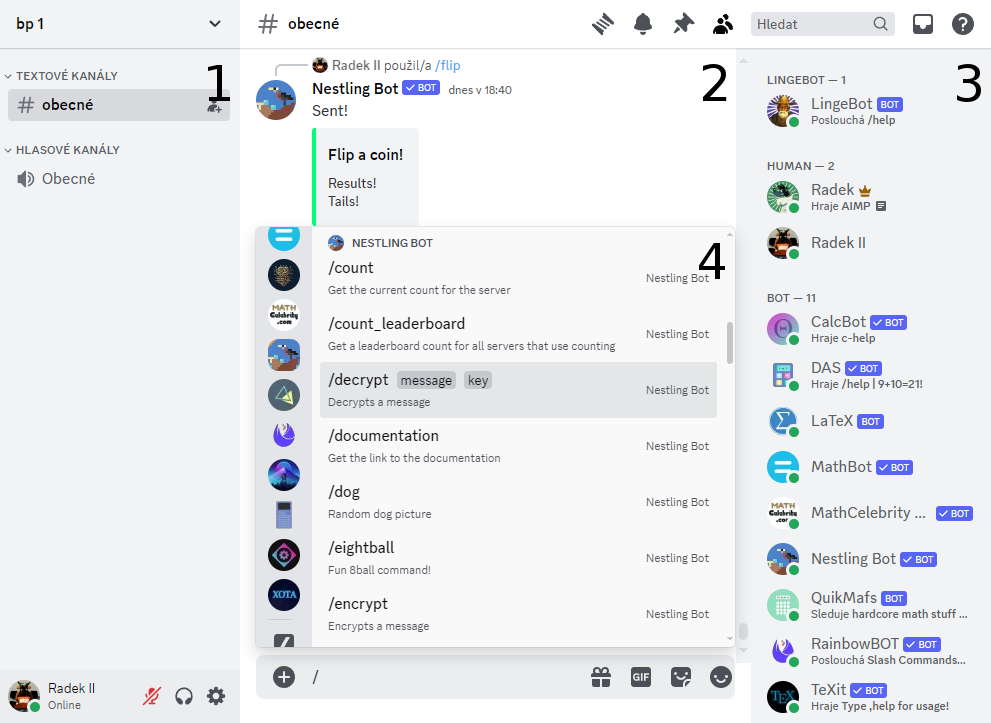
\includegraphics[width=\textwidth]{img/DiscordBotCommands}
		\caption{Discord: Uživatelské rozhraní a použití bota}
	\end{figure}
	
	Boti tedy operují především na serverech\footnote{Boty lze ale používat i v přímých zprávách. Bot se sice tváří jako uživatel, do přátel ho ale přidat nelze a pro zahájení přímé konverzace je nutné s ním nejdříve mít nějaký společný server. Bota nelze přidat do soukromé skupiny.} a existuje několik možností, jak je na nějaký server pozvat. Na konci roku 2022 byl do Discordu přidán tzv. adresář aplikací (\textit{App Directory}), který momentálně obsahuje seznam více než 5500 dostupných botů, kde každý z nich má svou stránku s podrobnějším popisem a tlačítkem pro přidání na server. Aby byl bot v tomto adresáři obsažen, musí nejprve projít schvalovacím procesem, a proto se jich zde nachází pouze zlomek ze všech existujících. Každý bot pak má svůj speciální zvací odkaz (\textit{bot invite link}) a existuje několik neoficiálních databází (např. \href{https://top.gg}{top.gg}), které opět obsahují seznam botů s jejich popisem a zvacím odkazem. Poslední možností jsou boti s otevřeným zdrojovým kódem, které si uživatel stáhne a spustí na vlastním stroji. Tento způsob vyžaduje botu založit účet a vygenerovat vlastní token.
	
	Discord boti nabízející nástroje pro usnadnění moderace zejména na velkých serverech patří mezi ty nejpoužívanější. Obvykle mají svou stránku s administrací, kde si lze např. zobrazit statistiky serveru, nastavit automatické přivítání a přiřazení rolí novým členům, vyhození za spam apod. Oblíbenou kategorií byli také hudební boti, kteří v hlasovém hovoru pouštěli vybrané skladby. Jejich popularita klesla roku 2021, kdy Google zakázal provoz botů přehrávajících hudbu z webu \mbox{YouTube}. Další častá kategorie botů jsou hry a zábava. Jedná se buď o boty poskytující jednoduché hry v prostředí textového chatu, nebo propojující nějakou existující videohru s Discordem.
	
	\section{Slack}
	
	Z populárních platforem se Discordu vzhledově i funkčně nejvíce podobá program Slack. Ten byl spuštěn již v roce 2013 a od té doby si vybudoval reputaci jako standard pro komunikaci v technologických společnostech. \cite{lit_Discord}
	
	Slack se prezentuje jako software usnadňující interní komunikaci v organizacích a dal by se nazvat jako ,,Discord pro firmy``. Namísto serverů jsou zde tzv. workspaces. Workspace má své členy a textové kanály, ve kterých lze zahájit i hlasový hovor. Členové jednoho workspace si mezi sebou mohou posílat přímé zprávy a pomocí funkce \textit{Slack Connect} je možné komunikovat i s lidmi z jiného workspace. Na rozdíl od Discordu, kde jsou přímé zprávy kompletně oddělené od ekosystému serverů, se zde všechny prováděné akce dějí uvnitř nějakého workspace.
	
	Slack má k dispozici několik úrovní měsíčního předplatného a verze zdarma je značně omezena. V bezplatné verzi nelze např. zobrazit zprávy starší než 90 dnů a provozovat hlasový hovor ve více než dvou lidech. Omezené je i použití tzv. aplikací.
	
	Zdejší aplikace (\textit{Apps}) se podobají zkoumaným botům a jejich výběr odpovídá cílové skupině Slacku. Zaměřují se především na zvýšení produktivity, \mbox{teambuilding}, nebo integraci již existující služby třetí strany do prostředí Slacku. Stejně jako uživatelé mohou Slack aplikace spravovat konverzace a odesílat do nich textové zprávy. Ovládání aplikací probíhá buď pomocí příkazů začínajících lomítkem, nebo má každá aplikace svou domovskou stránku a může také generovat vyskakovací okna. Aplikací odeslané zprávy, její domovská stránka a vyskakovací okna mohou obsahovat širokou škálu interaktivních prvků (tlačítko, zaškrtávací pole, výběr data a času apod.).
	
	\begin{figure}[ht]
		\centering
		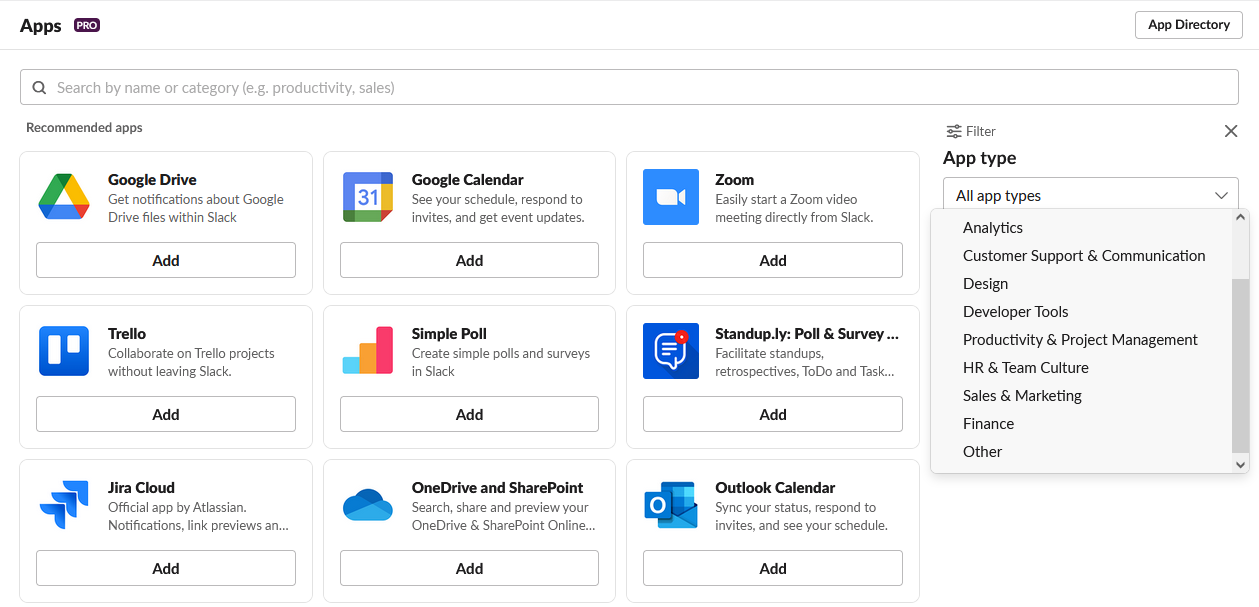
\includegraphics[width=\textwidth]{img/SlackApps}
		\caption{Doporučené Slack aplikace}
	\end{figure}
	
	Zorientovat se v procesu tvorby Slack aplikací nemusí být jednoduché. Tyto aplikace se totiž dělí na klasické (\textit{classic}) a nové (zvané \textit{modern} nebo \textit{next-generation}, představené v roce 2021), jejichž API se liší. Ani slovo bot není ve Slack ekosystému jednoznačné. U klasických aplikací se jedná o jejich speciální typ, se kterým je komunikace vedena běžnou řečí namísto příkazů nebo UI (chatbot). Tento bot je označen jako \textit{legacy} a v budoucnu pravděpodobně nebude podporován. U nového typu aplikací se z pohledu uživatele slovo bot nikde nevyskytuje (maximálně v názvu nějaké aplikace), z dokumentace je ale zjevné, že se (stejně jako u Discordu) jedná o speciálního uživatele ovládaného danou aplikací, tato informace však není nikde explicitně zmíněna. Při práci s dokumentací nebo neoficiálními návody je tedy nutné dávat pozor na to, s jakou technologií daný manuál pracuje, protože může dojít ke snadné záměně výše zmíněných pojmů.
	
	Klasické Slack aplikace lze vyvíjet v řadě komunitních knihoven. \textit{Next-generation apps} pak mají připravené oficiální \mbox{TypeScript} SDK a o hosting se stará přímo Slack, pro jejich vývoj a následné nasazení je ale nutné mít placenou verzi Slacku.
	
	\section{Guilded a Revolt}
	
	Guilded a Revolt jsou platformy, které jsou přímo inspirované Discordem a podobnost mezi nimi je nepřehlédnutelná. Ekosystém uživatelů, přímých zpráv, serverů a botů je u těchto tří platforem takřka identický. Guilded ani Revolt nemají ekvivalent k podpůrným příkazům. Boti tedy musí kontrolovat obsah každé odeslané zprávy na serveru, jestli neobsahuje nějaký z jejich příkazů. Každý bot má obvykle svůj prefix (např. vykřičník) a problém nastává, když má více botů stejný prefix a příkaz se stejným názvem (např. po napsání ,,!help`` do chatu zobrazí svou nápovědu všichni takoví boti)\footnote{Tímto způsobem se před představením podpůrných příkazů ovládali i boti na Discordu. Problém stejných příkazů se řešil buď víceznakovými prefixy (menší šance na kolizi), nebo nastavitelným prefixem (to vyžaduje nějaké úložiště uchovávající dvojice id serveru a prefix). Tento starý typ příkazů lze stále používat např. pokud je vývojář chce skrýt před běžnými uživateli (tyto příkazy se neobjeví v našeptávači).}. Obě platformy mají oproti Discordu znatelně menší uživatelskou základnu a počet jejich veřejných botů se pohybuje v řádu desítek.
	
	Guilded (2017) lze považovat za konkurenci Discordu, která se zaměřuje na jeho původní účel. Tím je komunikace pro hráče videoher. Guilded přidává funkce užitečné pro pořádání pravidelných komunitních událostí. Uživatel zde také může propojit svůj účet s vybranými herními tituly. \cite{web_guilded} 
	
	Program je zdarma, ale správci mohou na svém serveru zapnout dobrovolné měsíční předplatné, ze kterého je část odváděna Guilded. Pro tvorbu botů lze využít komunitních knihoven.
	
	Revolt (2021) je Discord alternativa s otevřeným zdrojovým kódem. Oproti konkurenci nemá Revolt žádné speciální funkce, díky tomu je ale méně komplikovaný. Kromě řady komunitních knihoven pro tvorbu botů je k dispozici i oficiální revolt.js. Tato knihovna byla vytvořena tak, aby do ní šel snadno migrovat bot napsaný v knihovně discord.js.
	
	\section{Další platformy}
	
	Do této sekce byly zařazeny další sociální platformy, které sice podporují implementaci botů ve smyslu automatizovaných uživatelů, ale oproti výše zmíněným platformám mají buď znatelně odlišnou strukturu a uživatelské rozhraní, nebo menší uživatelskou základnu, která se pak projevuje i v malém počtu existujících botů a malé komunitě kolem knihoven pro jejich tvorbu.
	
	\subsection{Matrix}
	
	Matrix je otevřený protokol pro šifrovanou a decentralizovanou komunikaci po síti. Existuje pro něj několik klientských aplikací (např. Element) a poskytovatelů (např. matrix.org). Protokol je také možné provozovat na vlastním serveru. Komunikace zde probíhá v tzv. místnostech. Místnost je jeden textový kanál s možností zahájení hlasového hovoru, který může být soukromý i veřejný. Pak jsou zde tzv. prostory, které jsou v podstatě jen spravované seznamy různých místností. Podle dokumentace jsou prostory podobné Discord serverům nebo Slack workspaces, avšak zde připojení do prostoru uživatele automaticky nepřipojí do všech místností (uživatel si může vybrat, kam se připojí) a místnosti nejsou na prostorech závislé (místnost může existovat bez prostoru, může ale být i součástí více prostorů). Matrix podporuje komunikaci uživatelů s různými poskytovateli tohoto protokolu ve stejné místnosti.
	
	Bot zde není speciálním typem uživatele, ale je pro něj zaregistrován běžný uživatelský účet. Program s logikou bota tedy může ovládat jakýkoliv účet (pokud zná jeho přístupový token)\footnote{V terminologii Discordu se běžné uživatelské účty řízené programem nazývají \textit{self-bots} a jejich provoz porušuje podmínky používání.}. Pro tvorbu takovýchto botů je připraveno oficiální \mbox{TypeScript} SDK. Veřejných botů pro Matrix není mnoho, mezi populární boty ale patří i boti modulární, do nichž mohou ostatní vývojáři přidávat vlastní funkcionalitu.
	
	Specifickou vlastností Matrixu jsou mosty (\textit{bridges}). Ty umožňují propojit místnost s nějakou jinou platformou (např. Discord, Slack nebo Messenger). Chat z platformy třetí strany by se pak měl zrcadlit s vybranou místností. Uživatelé z jiné platformy mají v Matrix místnosti svou reprezentaci zvanou \textit{ghost}. Pokud to daná platforma podporuje, tak v jejím ekvivalentu místnosti budou uživatelé ze strany Matrixu reprezentováni jako tzv. \textit{puppets}. \cite{doc_Matrix}
	
	\subsection{Microsoft Teams}
	
	Microsoft Teams je, stejně jako Slack, platforma pro firemní komunikaci. Každý účet na Teams náleží jedné organizaci (přihlašuje se obvykle přes firemní e-mail). Organizace se pak dělí na týmy, které se mohou dělit na kanály. Tým je kolekce uživatelů, která by měla reprezentovat určitý celek v dané organizaci (např. lidé pracující na konkrétním projektu). Kanály jsou sekce svého týmu, ve kterých probíhá komunikace ve formě příspěvků a komentářů. Klasický textový chat s případným hlasovým hovorem probíhá v samostatné sekci a umožňuje se spojit i s uživateli z jiné organizace.
	
	Podobně jako u Slacku se zdejší aplikace zaměřují především na zvýšení produktivity a propojení Teams s dalšími službami. Bot je v Teams terminologii aplikace vykonávající repetitivní úkony, která se může účastnit konverzace v chatu nebo kanálu. Boti se tvoří v oficiálním SDK (jazyky C\#, JavaScript, Python). Na konci roku 2023 bylo představeno Microsoft Copilot Studio, které mimo jiné podporuje tvorbu Teams botů pomocí grafického rozhraní bez psaní zdrojového kódu. Pro tento typ botů není potřeba vlastní hosting.
	
	Platforma Teams je součástí předplatného Microsoft 365. Existuje i bezplatná verze, ta má ale omezenou funkcionalitu a nedovoluje integraci aplikací (včetně botů). Kromě Teams pro firmy byla také později představena verze pro domácnosti. Ta by měla sloužit pro komunikaci s rodinou a přáteli. Většina funkcí je v této verzi vypnuta. Místo týmů jsou zde tzv. komunity, které se chovají totožně, pro jejich správu je ale nutné použít mobilní aplikaci.
	
	\subsection{Flock}
	
	Flock je platforma pro firemní komunikaci, která podle svého webu nabízí oproti konkurenčnímu Slacku a Teams více funkcí za méně peněz. Tento web obsahuje výčet více jak sta vlastností, ve kterých je Flock údajně lepší než konkurence. Po bližším průzkumu je ale zjevné, že některá uvedená tvrzení jsou nepravdivá nebo zavádějící.
	
	Struktura Flocku je podobná jako u ostatních platforem: Jednotlivé servery se nazývají týmy a obsahují textové kanály, ve kterých je možné zahájit hlasový hovor. Zdejší aplikace komunikují s Flock API a boti jsou jejich uživatelské reprezentace. Výběr aplikací je podobný jako u platforem Slack a Teams.
	
	Platforma pro vývoj Flock aplikací se nazývá FlockOS a má slogan ,,World's First Chat Operating System``, s operačním systémem ale nemá nic společného. Boty lze programovat v oficiálním SDK, jehož poslední verze ale vyšla v roce 2017.
	
	\subsection{Mattermost, Rocket.Chat a Zulip}
	
	Mattermost, Rocket.Chat a Zulip jsou komunikační platformy s otevřeným zdrojovým kódem. Díky tomu je možné provozovat tyto platformy na vlastních strojích (self-hosting), což je vhodné pro firmy, které díky tomu mají všechna data z chatů uložena u sebe. Všechny tři platformy ale nabízí i svůj hosting v několika úrovních měsíčního předplatného. Struktura těchto programů se pak podobá Slacku.
	
	Mattermost nemá žádnou knihovnu pro tvorbu botů, veškerou logiku komunikace s jejich API tedy musí zajistit vývojář bota. Pro Rocket.Chat je možné vyvíjet boty v oficiálním JavaScript SDK, nebo je vytvořit v grafickém rozhraní na platformě Botpress. Zulip má pro vývoj botů k dispozici oficiální Python knihovnu.
		
	\chapter{Matematika na platformě Discord}
	
	Ze zkoumaných sociálních platforem má Discord nejkomplexnější a nejlépe zdokumentovaný ekosystém botů. Kolem tvorby těchto botů vznikla početná komunita a existuje pro ni tedy i nejvíce knihoven. Discord nemá žádné specifické zaměření (např. firemní nebo herní) a díky tomu pokrývá širokou škálu uživatelů. Proto byla pro tvorbu matematického bota vybrána právě tato platforma.
	
	Ačkoliv nebyl Discord vytvořen pro účely výuky a nemá žádné speciální matematické nástroje, \textit{vzdělávání} je jednou z pěti hlavních kategorií veřejných Discord serverů a patří do ní i servery specializované na matematiku. \textit{Mathematics} je nejpopulárnější server s tímto zaměřením, na kterém mohou uživatelé diskutovat a řešit matematické problémy různých úrovní složitosti.
	
	Na serveru je také automatický systém přiřazování textových kanálů uživatelům s konkrétním matematickým problémem. Ostatní uživatelé se v daném kanále mohou pokusit zadaný problém vyřešit. Jakmile je zadavatelova otázka zodpovězena, textový kanál se může použít pro problém dalšího uživatele. O logiku přiřazování kanálů se stará místní bot.
	
	Matematicky zaměřených Discord botů není mnoho. V oficiálním adresáři aplikací nebyl během rešerše nalezen žádný. V neoficiálních databázích pak sice bylo nalezeno několik desítek botů, kteří se podle popisu alespoň částečně zabývají matematikou, velká část z nich ale byla offline a neměla k dispozici zdrojový kód. Otestováno bylo tedy nakonec 11 botů, které lze zařadit do dvou kategorií.
	
	\section{Bot vykreslující matematické výrazy}
	\label{_tag_section_texbot}

	Jelikož Discord nemá žádnou podporu pro vykreslování matematických výrazů, což je v textové konverzaci ohledně matematiky velmi užitečné, existuje hned několik botů s touto funkcionalitou. Konkrétně vykreslení umožňuje 5 z 11 testovaných botů. K popisu výrazu se ve všech případech používá TeX syntax, ve které je zadán vstupní parametr vykreslovacího příkazu. Bot pak podle parametru vygeneruje obrázek s matematickým výrazem a odešle ho do textového kanálu, kde byl příkaz zadán.
	
	Dva zkoumaní boti mají možnost zapnout automatické vykreslování: Jakmile jakákoliv odeslaná zpráva na serveru obsahuje dvakrát symbol dolaru, bot celou tuto zprávu vykreslí do obrázku a text mezi dolary nahradí matematickým zápisem (obrázek \ref{_tag_img_autotex}). Tři boti pak umožňují změnit barevné schéma generovaných obrázků. Je vhodné, aby tyto obrázky neměly průhledné pozadí, jinak by např. uživatelé používající světlý motiv Discordu nemohli přečíst text v obrázcích s bílou barvou písma (na průhledném pozadí).
	
	\begin{figure}[ht]
		\centering
		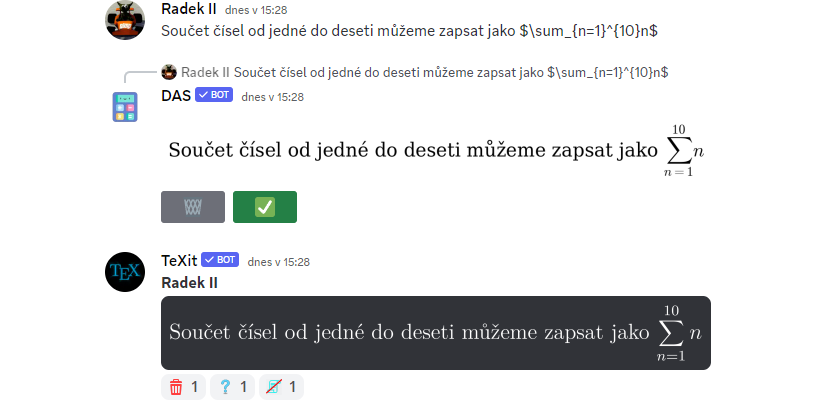
\includegraphics[width=\textwidth]{img/AutoTeX}
		\caption{Automatické vykreslení matematického výrazu}
		\label{_tag_img_autotex}
	\end{figure}
	
	U botů psaných v jazyce JavaScript lze pro implementaci této funkcionality využít knihovny KaTeX nebo MathJax. V jazyce Python to pak umožňuje Matplotlib. Tento balík sám o sobě ale neumí vykreslovat složitější prvky jako např. matice. K tomu je potřeba, aby na stroji, kde je bot spuštěn, byla nainstalována LaTeX distribuce, která se pak použije namísto výchozího Matplotlib vykreslování. Další možností nezávislou na použitém jazyku či knihovně je využít pro vykreslení nějakou externí službu.
	
	\section{Bot jako kalkulačka}
	
	Celkem devět otestovaných botů má jeden nebo více příkazů pro výpočet jednoduchých příkladů. V lepším případě se jedná o jeden příkaz (typu \textit{vypočti}), kterému se jako vstupní parametr zadá příklad s různými operacemi (včetně závorek, goniometrických funkcí apod.) a výstupem je výsledek celého výrazu. Velmi nepraktickou variantou jsou pak boti se sadou příkazů pro různé operace (typu \textit{sečti}, \textit{vynásob}, \dots), kde vstupem je několik čísel.
	
	Kromě výpočtu numerických příkladů se také objevují příkazy např. pro úpravy výrazů, derivace apod. Sedm botů pak dokáže vygenerovat obrázek s jednoduchým grafem dle zadaného předpisu. Dva boti umí zadat uživatelův vstup do služby Wolfram Alpha a do chatu odeslat její výstup.
	
	Jeden bot dokáže generovat náhodné příklady, jedná se ale pouze o čtyři základní binární operace. Tedy např. $x+y$, kde $x$ a $y$ jsou v rozmezí 1 až 99. Bot postupně generuje sérii deseti příkladů a uživatel má u každého deset vteřin na zadání výsledku. Po dokončení série příkladů je pak uživateli zobrazeno jeho skóre.
	
	% \section{DAS} ?
	
	\chapter{Prostředky pro tvorbu Discord bota}
		
	Discord API, se kterým program ovládající bota komunikuje, se dělí na dvě hlavní vrstvy: Pro obecné operace slouží HTTPS REST API a pro odesílání a přihlašování k událostem v reálném čase se používají trvalá zabezpečená připojení pomocí protokolu WebSocket. Samotná komunikace pak probíhá ve formátu JSON a pro unikátní identifikátory všech objektů se využívá formát Twitter Snowflake ID.	Discord operuje na tak velkém měřítku, že zajistit úplnou konzistenci jeho dat by bylo nemožné, a proto je většina operací v Discord API eventuálně konzistentní. \cite{doc_Discord}
	
	Eventuální konzistence znamená, že distribuovaná a replikovaná databáze povoluje relativně velké množství nekonzistentních dat. Pokud ale po nějaký čas neproběhne operace zápisu, tak se data na všech replikách postupně ,,srovnají``. \cite{book_distributedSystems4}
	
	Tvorba aplikací pracujících nad eventuálně konzistentními daty může být náročná. Události z Discord API navíc nemusí klientovi vždy přijít právě jen jednou, a proto je na ně nutné reagovat idempotentně. Výsledek několikrát provedené idempotentní operace by měl být stejný, jako kdyby byla provedena jen jednou. \cite{book_distributedSystemsUnderstanding}
	
	Z důvodu usnadnění tvorby Discord botů začaly pro tento účel vznikat komunitní knihovny. Oficiální dokumentace jich zmiňuje celkem 21 pro 11 různých programovacích jazyků. Tato kapitola blíže představuje některé z těchto knihoven, ve kterých byl v rámci rešerše implementován jednoduchý příkaz pojmenovaný \textit{pow}. Ten přijímá dva celočíselné parametry, se kterými provede umocňování. Ke zprávě s výsledkem je ještě přidáno tlačítko odkazující na webovou stránku (viz obrázky \ref{_tag_img_pow} až \ref{_tag_img_pow_last}).
	
	\begin{table}[ht]
		\centering
		\caption{Nejpopulárnější knihovny pro tvorbu Discord botů}\medskip
		\begin{threeparttable}
			\rowcolors{2}{gray!10}{}
			\begin{tabular}{ l l c c r }
				\textbf{Název} & \textbf{Jazyk} & \textbf{Vznik} & \textbf{Oficiální tutoriály} & \textbf{Popularita}\tnote{*} \\\hline
				discord.js	& JavaScript & 2015 & Ano & 24 452 \\
				discord.py	& Python	 & 2015 & Ne  & 14 024 \\
				DiscordGo	& Go		 & 2015 & Ne  &  4 563 \\
				serenity	& Rust		 & 2016 & Ne  &  4 259 \\
				JDA			& Java		 & 2015 & Ano &  4 038 \\
				Discord.Net & C\#		 & 2015 & Ano &  3 165 \\
				Pycord		& Python	 & 2021 & Ano &  2 619 \\
				Discord4J	& Java		 & 2015 & Ano &  1 697 \\
				Eris		& JavaScript & 2016 & Ne  &  1 465 \\
				DSharpPlus	& C\#		 & 2016 & Ano &  1 179 \\
			\hline\end{tabular}
			\begin{tablenotes}
				\item[*] počet GitHub hvězd ke dni 15. 2. 2024
			\end{tablenotes}
		\end{threeparttable}
	\end{table}
	
	\section{discord.py}
	\label{_tag_section_discordpy}
	
	Discord.py je knihovna pro tvorbu Discord botů v jazyce Python, která je distribuována v podobě balíku instalovaného programem pip. Pro definici veškeré funkcionality bota se využívá klíčových slov \verb|async| a \verb|await|. Bot je zde instancí předdefinované třídy s metodami, které se spouští při určité události a jejichž tělo lze dodefinovat. Pro přiřazení metod ke konkrétní události se často používají dekorátory, což je syntax umožňující upravit chování metod bez zásahu do jejich těla. Některé části discord.py (např. interaktivní prvky nebo tzv. \textit{cogs}) pak využívají objektového návrhu. 
	
	Cogs umožňují rozdělit logiku bota do více tříd, které dědí z třídy \textit{Cog} definované knihovnou. Každá taková třída je v discord.py terminologii zvaná cog a slouží jako kolekce souvisejících metod, které buď obsluhují příkazy, nebo reagují na události. Zvykem je, aby se každý cog nacházel ve zvláštním souboru a aby se každý z těchto souborů nacházel v adresáři pojmenovaném \textit{cogs}. Instance cog tříd jsou pak do bota nahrány nikoliv přes importování, ale pomocí mechanismu rozšíření (\textit{extensions}), který knihovna přidává. Za běhu programu je možné rozšíření přidávat a odebírat bez nutnosti restartování (\textit{hot reload}).
	
	Výhodou discord.py je jeho velká komunita, od které lze získat podporu např. na webu Stack Overflow nebo na oficiálním Discord serveru této knihovny. Díky použití dekorátorů (a jazyka Python obecně) může být psaný kód čitelný a zároveň mít vysokou hustotu. Pro definici příkazů lze navíc využít anotací a komentářů u příslušných metod. Knihovna má k dispozici referenční příručku, která stručně popisuje veškerou její funkcionalitu. Podrobnější popisy nebo příklady použití se zde ale vyskytují jen zřídka.
	
	Největším problémem discord.py je podle hlasování uživatelů na GitHub \mbox{Issues} absence oficiálních tutoriálů. Referenční příručka je dobrým nástrojem hlavně pro programátory, kteří už obecnou tvorbu botů v této knihovně ovládají, a neobsahuje např. informace o tom, jak strukturovat větší projekt nebo co znamenají jednotlivé funkce knihovny z pohledu koncového uživatele.
	
	V roce 2021, kdy byly mimo jiné představeny podpůrné příkazy, vyšla nová verze Discord API, která přinesla zásadní změny v jeho používání. To vedlo k frustraci autorů některých knihoven a vývoj discord.py byl pozastaven. Po šesti měsících se repozitář opět otevřel a vývoj mohl pokračovat, mezitím ale vzniklo několik nových knihoven založených na discord.py (konkrétně Pycord, Nextcord a disnake). Zároveň začaly vycházet balíky, které do existující knihovny přidávaly podporu pro novou verzi Discord API. Zdrojové kódy těchto knihoven jsou si velmi podobné, a proto je při hledání informací nutné dávat pozor na to, s jakou knihovnou daný zdroj pracuje.
	
	\section{discord.js}
	
	Discord.js je knihovna pro běhové prostředí Node.js umožňující tvorbu Discord botů v jazycích JavaScript nebo TypeScript. Funkcionalita je založena na objektech \verb|Promise| a při psaní kódu se využívá tzv. arrow funkcí. Režie pro zprovoznění podpůrných příkazů a modularity (zde ve stylu \textit{co soubor, to příkaz}) je o něco složitější než u discord.py.
	
	Velkou výhodou této knihovny je existence oficiálních tutoriálů, které programátora provedou krok za krokem od úvodní instalace npm balíčku až po tvorbu pokročilých příkazů. Krom popisu postupů a zdrojových kódu se díky tomuto návodu programátor rychle dozví, co všechno do svého bota vlastně může implementovat. Nechybí ani referenční příručka a početná komunita jako u discord.py.
	
	Knihovna nevyužívá dekorátorů ani komentářů pro definování příkazů. Výsledný kód obsahuje mnoho vnořených nebo zřetězených funkcí, kvůli kterým může být delší a hůře čitelný. Knihovna sice podporuje TypeScript, oficiálních ani komunitních návodů pro jeho korektní použití ale není mnoho.
	
	\section{Discord.Net}
	
	Discord.Net je knihovna pro tvorbu Discord botů na platformě .NET, kterou lze do projektu přidat přes systém NuGet. Dokumentace je psaná pro jazyk C\#, ve kterém je tato knihovna implementována. Pro tvorbu bota je ale možné použít i jiné jazyky z této platformy jako F\# nebo Visual Basic. Knihovna má k dispozici referenční příručku i tutoriály, její nevýhodou je menší komunita.
	
	 Pro tvorbu složitějších botů se doporučuje použít vkládání závislostí\footnote{Vkládání závislostí (\textit{dependency injection}) je návrhový vzor, kde se třetí strana stará o vztahy mezi komponentami a jejich závislostmi (aby byla za běhu programu do vybraných atributů dosazena správná instance) \cite{lit_distributedSystems}. Zde se konkrétně jedná o balík \textit{Microsoft.Extensions.DependencyInjection}.}. Oproti předchozím knihovnám Discord.Net u podpůrných příkazů odděluje logiku jejich synchronizace a obsluhy. Kód zde tedy není strukturován na metody odpovídající jednotlivým příkazům, ale všechny příkazy jsou obsluhovány jedinou metodou, ve které je kód dále rozvětven\footnote{Podpůrné příkazy musí být synchronizovány, aby je mohli uživatelé používat. V discord.py a discord.js jsou všechny potřebné informace pro synchronizaci (jméno, popis a vstupní parametry) součástí definice obslužné funkce daného příkazu. V Discord.Net jsou tyto informace uvedeny ve speciální metodě pro synchronizaci. Druhá speciální metoda pak obsluhuje všechny příkazy. Obvykle je uvnitř druhé metody rozvětvení typu \textit{switch} podle jména příkazu.}.
	
	\section{JDA}
	
	JDA je knihovna pro tvorbu botů v jazyce Java nebo Kotlin. Do projektu je přidána pomocí nástroje Maven nebo Gradle. Stejně jako u Discord.Net je zde oddělená logika synchronizace podpůrných příkazů s Discordem od jejich samotné obsluhy.
	
	Referenční příručka JDA je vygenerována přes Javadoc, což může být vhodné pro programátory zvyklé na jazyk Java, na první pohled ale působí složitě a nepřehledně. K dispozici jsou také tutoriály včetně ukázkové implementace bota přehrávajícího hudbu v hlasovém hovoru. Ze čtyř zkoumaných knihoven se jedná o jedinou, která by takto v návodu obsahovala krok za krokem kompletní proces tvorby bota s konkrétním zaměřením.
	
	\chapter{Tvorba matematického Discord bota}
	
	Tato kapitola popisuje tvorbu matematického Discord bota, který byl pojmenován \textit{LingeBot}. Zaměřuje se na výklad teorie a generování příkladů z lineární algebry. K výkladu této látky lze přistupovat s různou mírou obecnosti: Některé zdroje prezentují lineární algebru jako sadu postupů pro řešení určitých matematických úloh, jiné ji vykládají jako teorii vektorových prostorů a lineárních zobrazení \cite{lit_lingebra}. Bot byl vytvořen spíše pro prezentování informací z druhé zmíněné strany spektra, avšak jeho návrh obecně podporuje jakýkoliv typ matematických materiálů. Generované příklady se pak soustředí na základní výpočty s maticemi.
	
	Pro tvorbu bota byla zvolena knihovna discord.py zejména kvůli její početné komunitě a čitelnosti výsledného zdrojového kódu. Při volbě také hrála roli existence matematických knihoven pro jazyk Python (konkrétně Matplotlib, NumPy, SciPy a SymPy), které jsou zavedené a dobře zdokumentované.
		
	\section{Návrh}
	
	\subsection{Vykreslení matematických výrazů}
	
	Jak již bylo zmíněno v sekci \ref{_tag_section_texbot}, pro textovou komunikaci ohledně matematiky je vhodné používat správné matematické symboly. Příkladem je situace, kdy chce jeden uživatel odeslat a popsat druhému uživateli vzorec obsahující mocniny (např. $x^2$). Pokud si uživatel nepamatuje specifický alt kód, pak symbol ,,$^2$`` není možné na klávesnici napsat. Ne příliš praktickým řešením je najít a zkopírovat daný symbol buď z internetu, nebo programu jako je \textit{mapa znaků}. Další možností je zavést alternativní značení, tedy např. místo $x^2$ psát $x$\textsuperscript{$\wedge$}2 nebo $x$**2. Tato značení ale nejsou nijak normalizovaná a v textové konverzaci zejména více uživatelů mohou vést k nedorozuměním. Obě možnosti navíc selhávají ve chvíli, kdy je potřeba zapsat buď velké množství různých symbolů, nebo složitější výrazy obsahující zlomky, matice atd. Některá textová prostředí podporují vykreslování HTML: Pro horní a dolní index lze využít značek \verb|sup| a \verb|sub|, řecká písmena lze pak psát např. jako \verb|&alpha;|. Pro jakýkoliv složitější matematický výraz je ale jediným zavedeným způsobem program TeX a jeho syntax.
	
	Protože Discord vykreslování TeX výrazů nepodporuje, jedná se o jednu z funkcionalit navrhovaného bota. Konkrétně jde o příkaz \verb|/render| (\textit{vykresli}), jehož parametrem je právě matematický výraz zapsaný v TeX (resp. Matplotlib Mathtext) syntaxi, který má být vykreslen. Po spuštění příkazu je do chatu odeslán obrázek obsahující vykreslení požadovaného výrazu. Pod tímto obrázkem se nachází trojice tlačítek \textit{Potvrdit}, \textit{Upravit} a \textit{Smazat}. Tlačítko pro smazání kompletně odstraní botem odeslanou zprávu. Tlačítkem pro úpravu se vyvolá vyskakovací okno s textovým polem, ve kterém je předvyplněn uživatelův původní vstup. Po opravě nebo rozšíření výrazu je daný obrázek překreslen. Pokud se ve vstupu od uživatele nachází chyba, pak zpráva místo obrázku obsahuje výpis z chybového hlášení, díky kterému může uživatel chybu snadněji detekovat. Tlačítko potvrzení pouze nechá trojici tlačítek zmizet a tedy znemožní výraz dále upravovat nebo ho smazat. Tato akce se po určitém časovém intervalu provede automaticky, aby tlačítka zbytečně neznepřehledňovala textovou konverzaci.
	
	Vykreslování matematických výrazů je stěžejní funkcionalitou navrhovaného bota. Kromě příkazu \verb|/render| totiž může být použito i během výkladu teorie nebo při zobrazování vygenerovaných příkladů.
	
	\subsection{Výklad teorie}
	
	Výklad teorie funguje na principu odesílání zpráv obsahujících předem připravené výpisky z určitého tématu. Je dostupný pod příkazem \verb|/explain| (\textit{vysvětli}), po jehož zadání je uživateli zobrazen výběrový seznam všech dostupných témat. Každé téma odpovídá jednomu textovému souboru, aby nebyly výpisky součástí zdrojového kódu a bylo snazší je upravovat. Obsah souborů je psaný v jazyce Markdown, který Discord v textových zprávách podporuje a tedy umožňuje jejich formátování.
	
	Jazyk Markdown nemá žádnou oficiální syntax pro označení matematických výrazů, zvykem ale je výraz uzavřít z obou stran řetězcem tvořeným dvěma symboly dolaru (,,\verb|$$|``, dále jen ,,dvoudolar``). Pokud se tedy ve výpiscích nachází text ohraničený dvoudolary, pak je tato část do textového kanálu odeslána jako obrázek (podobně jako u příkazu \verb|/render|). Maximální délka odeslané zprávy na Discordu je 2000 znaků, a proto je bot schopen odesílané výpisky rozdělit do více zpráv. %Rozdělování do více zpráv je nutné právě i pro kombinování zpráv textových a těch obsahující obrázek.
	
	Každé teoretické téma (a tedy soubor) se dělí na několik podtémat, jejichž názvy a rozdělení jsou určeny podle nadpisů druhé úrovně v Markdown souboru. Po zvolení tématu z výběrového seznamu je do chatu odeslán seznam příslušných podtémat, mezi kterými lze přepínat pomocí tlačítek \textit{Další} a \textit{Předchozí}. V textovém kanálu se tedy vždy nachází zprávy patřící k aktuálně vybranému podtématu, které jsou po stisknutí jednoho z tlačítek smazány a nahrazeny novými. K flexibilnějšímu přepínání mezi podtématy byl přidán další výběrový seznam, z nějž lze vybrat jakékoliv podtéma a není nutné je procházet popořadě jako při použití tlačítek. Dalšími tlačítky u rozhraní výkladu teorie jsou \textit{Odeslat do DMs} (přepošle uživateli zprávy k danému podtématu do přímých zpráv), \textit{Ukončit} (nechá zmizet tlačítka, odeslané zprávy zůstanou) a \textit{Ukončit a smazat} (tlačítka i zprávy jsou odstraněny). Pokud konverzace s botem již probíhá v přímých zprávách (namísto serveru), pak tlačítko \textit{Odeslat do DMs} není dostupné.
	
	Během návrhu se původně uvažovalo o možnosti nahrávání nových témat uživateli. Discord umožňuje jako parametr příkazu předat soubor a uživatel by takto mohl do bota nahrát vlastní Markdown zápisky. Tento návrh ale otevírá několik otázek: Budou si moct nahrané zápisky zobrazit všichni uživatelé, nebo jen členové stejného serveru? Má být nastaven limit maximálního počtu nahraných souborů na konkrétního uživatele, nebo na server? Jak se stavět k nevhodnému obsahu? Navíc by bylo potřeba rozhraní, kde by uživatel mohl své nahrané soubory spravovat. To by v prostředí textového chatu nebylo příliš praktické, vhodnější by bylo k botu ještě vytvořit webové rozhraní.
	
	Nakonec byl zvolen přístup, kde si každý uživatel může provozovat vlastní instanci navrhovaného bota. Soubory s tématy jsou pak nakopírovány do vyhrazeného adresáře, odkud mohou být snadno spravovány. %TODO jak?
	
	\subsection{Generace příkladů} % kalkulačka zavržena
	
	Příklady lze generovat použitím příkazu \verb|/generate|, po jehož zadání je do textového kanálu opět odeslán výběrový seznam, který tentokrát obsahuje dostupné kategorie příkladů. Po volbě některé z kategorií se objeví trojice tlačítek \textit{Generovat příklad}, \textit{Jak počítat?} a \textit{Změnit kategorii / Ukončit}. Po vygenerování příkladu jej bot bez výsledku odešle do chatu. Uživatel si může zkusit příklad vypočítat, a poté si nově objeveným tlačítkem nechat zobrazit výsledek. Tento proces lze opakovat, dokud není rozhraní ukončeno.
	
	Navrhovaný bot neobsahuje funkcionalitu pro kontrolu uživatelem zadaných výsledků. Pokud by takovým výsledkem byla např. matice většího rozměru, její zadávání by bylo zdlouhavé a náchylné na překlepy. Muselo by také mít nastavená jasná pravidla zápisu, nebo by uživatelský vstup musel projít komplexnější syntaktickou analýzou. Pokud se uživatel dozví, že jeho výsledek je nesprávný, dalším krokem by mělo v každém případě být nalezení chyby a poučení se z ní. Znalost výsledku sice může hledání chyby trivializovat, avšak frustrace z nesprávných výsledků u uživatelů pravděpodobně stejně vede k okamžitému zobrazení těch správných.
	
	Po stisknutí tlačítka \textit{Jak počítat?} jsou do textového kanálu odeslány zprávy s návodem pro výpočet příkladů z dané kategorie. Logika odesílání těchto zpráv je stejná jako u výkladu teorie. Obsah je tedy čerpán z Markdown souborů, které lze snadno upravovat, a nechybí tlačítko pro přeposlání návodu do přímých zpráv. Každá kategorie příkladů nemusí nutně obsahovat návod, pak je tlačítko pro jeho zobrazení zašedlé a nelze s ním interagovat. Opačný stav, kdy existuje pouze návod a nelze generovat příklady, je také možný. % TODO (???)
		
	\subsection{Možnosti moderace}
	
	Aby byly demonstrovány specifické vlastnosti platformy Discord, byla do bota přidána funkcionalita pro moderaci (administraci) pomocí sady příkazů \verb|/setup|. Administrátoři serveru mohou u každého příkazu nastavit, kdo má oprávnění jej používat. Lze vybrat ze tří kategorií: pouze administrátoři, administrátoři a moderátoři bota, nebo kdokoliv (výchozí stav). Tato nastavení dávají smysl pouze při používání bota na serverech a v přímé konverzaci nemají význam.
	
	\textit{Administrátor} je typ oprávnění, které je součástí Discordu a uživatelům ho lze přidělit v rámci role. Pokud není taková role nikomu přidělena, pak je majitel serveru jediným uživatelem s těmito právy (a zároveň jediným, kdo může tuto roli někomu dalšímu přidělit).
	
	Za ,,moderátora bota`` je považován uživatel, kterému byla administrátorem přidělena speciální role s názvem \textit{LingeMod}. Tato role je vytvořena navrhovaným botem po jeho připojení na nový server. Díky moderátorské roli lze uživatele bez administrátorských práv rozdělit na dvě skupiny a pouze jedné z nich povolit používání určitých příkazů.
	
	Nastavení může vypadat např. následovně: Kdokoliv může vykreslovat matematické výrazy pomocí \verb|/render|, pouze moderátoři bota (a tedy i administrátoři, kteří jim jsou nadřazeni) mohou generovat příklady pomocí \verb|/generate| a pouze administrátoři mohou používat výklad teorie příkazem \verb|/explain|.
	
	Podobná oprávnění lze nastavit i u tlačítek a výběrových seznamů, které jsou součástí botem odeslaných zpráv. Ve výchozím stavu s nimi může interagovat pouze uživatel, na něhož je zpráva s interaktivními prvky mířena (zadavatel daného příkazu). Interakci s ,,cizími`` ovládacími prvky je ale možné povolit jakémukoliv administrátorovi nebo i moderátorovi bota. Tlačítko pro přeposlání daného podtématu do přímých zpráv je vždy dostupné všem.
	
	\subsection{Další funkcionalita} % $> old_commands
	
	Navrhovaný bot obsahuje příkaz \verb|/help| pro zobrazení stručné nápovědy. Zvykem při tvorbě Discord botů je také přidání příkazu \verb|/ping|, pomocí kterého lze otestovat, zdali je bot online. Příkaz ping je inspirován stejnojmenným programem a odpověď na něj obvykle vypisuje dobu odezvy (latenci) daného bota. V tomto případě byly do výpisu přidány i další informace jako doba provozu (uptime) nebo počet serverů, na kterých se navrhovaný bot nachází.
	
	Dalším přidaným příkazem, který byl inspirován prostředím terminálu, je \verb|/clear|. Po jeho zadání bot do chatu odešle  prázdnou zprávu, která je tak dlouhá, aby se všechny předchozí zprávy již nevešly na obrazovku. To může být užitečné pro zpřehlednění konverzace v daném textovém kanále.
	
	U bota je možné změnit barevné schéma vykreslovaných matematických výrazů. Konkrétně jsou k dispozici čtyři kombinace barvy písma a pozadí u odeslaných obrázků. Barevné schéma je vázané na server a může být přenastaveno jeho administrátorem. Všechny botem odeslané obrázky na určitý server budou respektovat jeho nastavené schéma nezávisle na uživateli příkazu. Uživatel si totiž může nastavit barevné schéma pro konverzaci s botem v přímých zprávách. To je použito u zpráv reagujících na příkazy spuštěné v přímé konverzaci a zároveň u zpráv přeposlaných z jakéhokoliv serveru pomocí tlačítka \textit{Odeslat do DMs}.
	
	\section{Implementace}
	
	\subsection{Struktura projektu}

	Před implementací jednotlivých funkčních částí výsledného bota bylo nutné rozhodnout, jak bude projekt strukturován. U knihovny discord.py je toto rozhodnutí ponecháno především na vývojáři: Dokumentace knihovny neobsahuje doporučený způsob, jak kód bota rozdělovat do více souborů, ani ukázku většího projektu, kterým by se dalo inspirovat.
	
	Zvyk ohledně cog souborů (viz \ref{_tag_section_discordpy}) byl během implementace bota dodržen. Logika vykonání příkazů ale byla ve většině případů oddělena do jiných souborů, které se v pomyslné hierarchii projektu nachází na jiné úrovni. Cogs je pak importují a pouze volají jejich metody. Podle toho, zdali jsou tyto ,,jiné`` soubory závislé na knihovně discord.py, je lze rozdělit do dvou skupin.
	
	Soubory, jež Discord knihovnu importují, ale nejedná se o cogs, se nachází v adresáři \textit{d\_modules}. Je v nich implementována logika, která je společná pro více příkazů, jako je kontrola oprávnění pro spuštění příkazu nebo odesílání a mazání textových zpráv. Zároveň se zde nachází veškerá logika pro obsluhu interaktivních prvků jako tlačítek a vyskakovacích oken, ale i modul obsahující definici samotného bota.
	
	Druhá skupina souborů, které neimportují discord.py, se nachází v adresáři \textit{utils}. Metody těchto modulů jsou importovány a používány především v \textit{d\_modules} pro společnou funkcionalitu, která je nezávislá na Discordu. Tyto moduly naopak importují knihovny jako sqlite, Matplotlib nebo SymPy a starají se tedy o práci s databází, vykreslování matematických výrazů nebo generování příkladů. % šly by teoreticky použít v jiné aplikaci, problems dostaly vlastní adresář a balík(?)
	
	Vedle těchto adresářů se ještě nachází soubory \textit{config.json} (uložení tokenu bota), \textit{db\_init.py} (vytvoření databáze), \textit{run.py} (spuštění bota) a adresáře \textit{\_database}, \textit{\_logs} a \textit{\_static}. Adresář \textit{\_static} obsahuje Markdown soubory s výpisky z teorie a návody pro počítání příkladů. % nic moc odstavec
	
	\begin{figure}[ht]
		\centering
		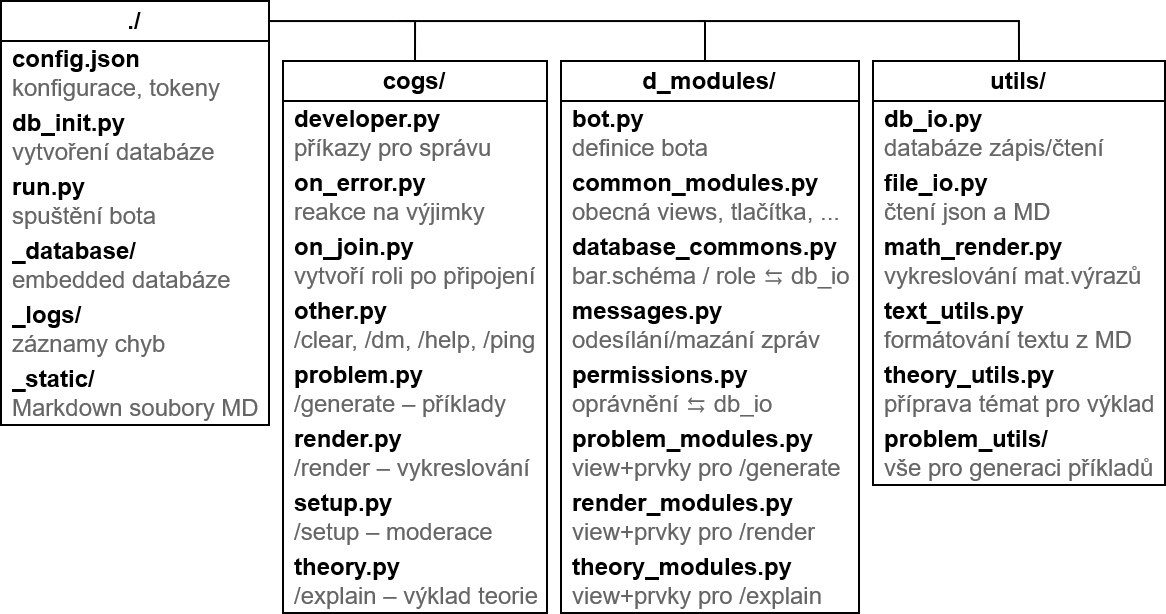
\includegraphics[width=\textwidth]{img/ProjectStructure}
		\caption{Struktura projektu}
	\end{figure}

	\subsection{Implementace vykreslování matematických výrazů}

	První verze implementace příkazu \verb|/render| byla prostá. Pomocí balíku Matplotlib je vytvořen prázdný obrázek \textit{figure}, jehož barva odpovídá barvě pozadí Discord klienta ve výchozím nastavení. Parametr příkazu, který obsahuje předpis matematického výrazu, je do obrázku vložen jako text se zapnutým parametrem \textit{render\_math}. Balík Matplotlib se postará o správné vykreslení výrazu a obrázek je uložen do souboru, který je následně odeslán do textového kanálu. Později bylo ukládání do souboru nahrazeno proudem \textit{io.BytesIO}, který souborové rozhraní pouze simuluje.

	Výklad lineární algebry se neobejde bez vykreslování matic, ty ale Matplotlib Mathtext nepodporuje. Balík sice umožňuje nastavit, aby vykreslování používalo místní TeX distribuci, během implementace ale nebylo jasné, kde bude výsledný bot nasazen a jestli zde bude možné TeX nainstalovat. Vykreslování tímto způsobem je navíc pomalejší. Proto byla pro účely bota napsána vlastní logika vykreslování matic.
	
	U textu vkládaného do Matplotlib obrázku lze nastavit i jeho souřadnice $x$ a $y$. Matice na vstupu implementované vykreslovací funkce je rozdělena na své jednotlivé prvky, které jsou vykresleny zvlášť na odpovídajících souřadnicích. Pomocí úseček jsou pak vytvořeny hranaté závorky matice. Problém může nastat při určování souřadnic jednotlivých prvků v matici.
	
	Pokud jsou všechny prvky matice jednociferná čísla, pak jejich souřadnice $x$ odpovídá číslu sloupce a $y$ číslu řádku v matici. Tyto souřadnice jsou ještě vynásobeny konstantou, která určuje velikost mezery mezi jednotlivými prvky\footnote{Konstanta u souřadnic $y$ by měla být záporná, protože řádky matice jsou obvykle číslovány odshora, zatímco souřadnice v Matplotlib obrázku mají počátek vlevo dole. V této implementaci je to ale vyřešeno tak, že se jednotlivé řádky matice při vykreslování procházejí pozpátku.}. Jakmile by ale byl některý z prvků matice širší (např. trojciferné číslo), začal by se překrývat se svými sousedními prvky. Proto je potřeba přidat funkcionalitu, která dokáže zjistit šířku prvku v matici. Odsazení je pak nastaveno podle nejširšího nalezeného prvku.
	
	Šířku prvku lze určit jeho dočasným vykreslením do samostatného obrázku, u kterého jsou následně zjištěny jeho rozměry. Tento obrázek je opět uložen do proudu BytesIO, který je po zjištění šířky zahozen. Takovýto způsob není nejefektivnější (zejména u vykreslování větších matic), a proto byla implementována rychlejší metoda, která šířku prvků pouze aproximuje.

	Cílem metody je pro zadaný matematický výraz v TeX syntaxi vrátit číslo, které odpovídá jeho délce. Jednotkou délky je počet nejkratších znaků. Písmo vykreslených matematických výrazů je totiž proporcionální a některé znaky tedy mohou být širší než jiné. Za nejkratší znaky se v tomto případě považují číslice a většina malých písmen. Protože se jedná pouze o aproximaci, je důležité, aby metoda délku výrazu přeceňovala. Podcenění by opět vedlo k překrývání sousedních prvků matice.
		
	\begin{figure}[ht]
		\begin{lstlisting}[language=Pseudo1]
Funkce __approx_tex_len(text: str, nahradit_zlomky: bool) vrací int:
Krok 1:
	Pokud nahradit_zlomky:
		Nahraď všechny výrazy v text ve tvaru "\frac{Č}{J}"
		za výstup funkce __approx_tex_frac_replace(Č, J).
Krok 2:
	Nahraď všechny podřetězce v text,
	které začínají na "\" a končí libovolným nepísmenným znakem,
	za dvouznakový řetězec "00".
Krok 3:
	Nahraď všechny znaky v text,
	které se zároveň nachází v "+-=ABCDEFGHKMNOPQRUVWXYZmw",
	za dvouznakový řetězec "00".
Krok 4:
	Odstraň všechny znaky z text,
	které se zároveň nachází v " _^{}[]".
Krok 5:
	Vrať délku upraveného řetězce text.
	
Funkce __approx_tex_frac_replace(čitatel, jmenovatel: str) vrací str:
	délka_čitatele = __approx_tex_len(čitatel, false)
	délka_jmenovatele = __approx_tex_len(jmenovatel, false)

	Vrať řetězec tvořený znaky "0"
	o délce maximum(délka_čitatele, délka_jmenovatele).
		\end{lstlisting}
		\caption{Pseudokód aproximace délky vykresleného výrazu}
	\end{figure}
	
	\newverbcommand{\h}{\color{color_cyan!95!black}}{}
	\begin{table}[ht]
		\centering
		\caption{Příklady aproximace délky vykresleného výrazu}\medskip
		\begin{tabular}{ l | l >{\columncolor{gray!10}}l l }\hline
			&&&\\[-1em]
			\textbf{Krok 1}&\verb|1+\sqrt{t}|&\verb|1+\sqrt[N]{t}|&\verb|t^2\approx|\h|\frac{123}{4}|\\
			&\verb|1+\sqrt{t}|&\verb|1+\sqrt[N]{t}|&\verb|t^2\approx|\h|000|\\\hline
			&&&\\[-1em]
			\textbf{Krok 2}&\verb|1+|\h|\sqrt|\verb|{t}|&\verb|1+|\h|\sqrt|\verb|[N]{t}|&\verb|t^2|\h|\approx|\verb|000|\\
			&\verb|1+|\h|00|\verb|{t}|&\verb|1+|\h|00|\verb|[N]{t}|&\verb|t^2|\h|00|\verb|000|\\\hline
			&&&\\[-1em]
			\textbf{Krok 3}&\verb|1|\h|+|\verb|00{t}|&\verb|1|\h|+|\verb|00[|\h|N|\verb|]{t}|&\verb|t^200000|\\
			&\verb|1|\h|00|\verb|00{t}|&\verb|1|\h|00|\verb|00[|\h|00|\verb|]{t}|&\verb|t^200000|\\\hline
			&&&\\[-1em]
			\textbf{Krok 4}&\verb|10000|\h|{|\verb|t|\h|}|&\verb|10000|\h|[|\verb|00|\h|]{|\verb|t|\h|}|&\verb|t|\h|^|\verb|200000|\\
			&\verb|10000t|&\verb|1000000t|&\verb|t200000|\\\hline
			&&&\\[-1em]
			\textbf{Krok 5}&6&8&7\\\hline
			&&&\\[-1em]
			\textbf{Porovnání}&$1+\sqrt{t}$&$1+\sqrt[N]{t}$&$t^2\approx\frac{123}{4}$\\
			&$123456$&$12345678$&$1234567$\\
		\hline\end{tabular}
	\end{table}
	
	Aproximovaná délka vykresleného výrazu odpovídá počtu znaků vstupního řetězce po tom, co je na něm provedeno několik úprav. Kroky 2 a 3 nahrazují určité části textu řetězcem s dvěma nulami. To, že je nahrazujícím znakem nula, není podstatné. Důležité je, že jsou nuly právě dvě. Následující krok odebere řídící znaky a mezery, pak už je vrácena délka řetězce.
	
	Při určování délky jsou problémové zlomky psané jako \verb|\frac{Č}{J}|. V nejhorším případě, pokud je délka čitatele \textit{\texttt{Č}} i jmenovatele \textit{\texttt{J}} stejně dlouhá, by byla šířka zlomku vyhodnocena jako dvojnásobek té skutečné. Proto byl přidán krok 1, ve kterém se metoda rekurzivně volá na všechny zlomky ve vstupním řetězci. Ty jsou pak nahrazeny řetězcem o aproximované délce jejich čitatele, nebo jmenovatele.

	Stejný problém jako zlomky také způsobují kombinační čísla \verb|\binom{N}{K}|, ta se ale běžně v maticích nenachází. Popisovaná metoda by šla dále vylepšovat pro mnoho dalších případů, které by mohly nastat. Jelikož ale byla navržena pro určování šířky prvků v matici, všechny časté scénáře by již měly být pokryté. % \iota

	Jelikož je pro vykreslování matic použita vlastní implementace, bylo možné zvolit styl jejich zápisu. Pro svou přehlednost, snadné strojové zpracování a rychlost zápisu uživatelem byla zvolena syntax podobná maticím v prostředí MATLAB: Do hranatých závorek jsou postupně vypsány prvky matice oddělené čárkou a pro oddělení jednotlivých řádků se místo čárky píše středník.

	Po implementaci metod pro vykreslení základních matematických výrazů a matic bylo potřeba tyto metody zkombinovat, aby bylo možné vykreslovat rovnice obsahující více matic. Uživatelský vstup je nejprve nutné rozdělit na maticové a nematicové části (podvýrazy), pro jejichž vykreslení je pak zvolena příslušná metoda. První podvýraz je vykreslen na nulové souřadnici $x$, která se postupně zvětšuje o aproximovanou délku podvýrazu. Při rozdělování na podvýrazy je nutné ignorovat hranaté závorky u odmocnin, maticový podvýraz je totiž detekován podle hranatých závorek. Aby byl celý výraz správně vertikálně zarovnán, je potřeba předem zjistit počet řádků té nejvyšší matice a podle ní určovat souřadnici $y$ zbylých podvýrazů.
	
	Posledním krokem bylo přidání podpory pro víceřádkové výrazy zarovnané podle určitého znaku. Obvykle se zarovnává podle rovnítka. Pomocí dvou zpětných lomítek je v uživatelském vstupu označen nový řádek. Na každém řádku lze zapsat ampersand, který není vykreslen ve výsledném obrázku a značí, že následující symbol je ten zarovnávací. Každý řádek je podle ampersandu rozdělen na levou a pravou část. Obě tyto části jsou vykresleny na nulové souřadnici $x$, u té levé je ale nastaveno Matplotlib zarovnání vpravo pomocí parametru \textit{horizontalalignment}.
	
	Vlastní metoda pro vykreslování matic ale nepočítá s přenastavováním zarovnání na úrovni balíku Matplotlib. Pokud se tedy ve zpracovávaném řádku nachází matice, pak je jeho levá část zarovnána pomocí metody pro aproximaci délky výrazu: Matplotlib zarovnání je ponecháno za výchozí hodnotě vlevo a souřadnice $x$ je rovna záporné aproximované délce. V opačném případě, kdy se v řádku žádné matice nevyskytují, je krok s rozdělováním na podvýrazy přeskočen a rovnou se sází Matplotlib Mathtext.
	
	\subsection{View a interaktivní prvky}
	
	K odeslané zprávě s vykresleným matematickým výrazem je přidána trojice tlačítek \textit{Potvrdit}, \textit{Upravit} a \textit{Smazat}. Aby mohl být ke zprávě přidán jakýkoliv interaktivní prvek, musí být nejprve vytvořeno tzv. view. To slouží jako kontejner pro všechny interaktivní prvky a ke zprávě je přidáno přes stejnojmenný parametr (viz obrázek \ref{_tag_img_discordpy}). Pro definici složitější view logiky je možné vytvořit třídu, která dědí z obecného view. Do této třídy se pak přidají atributy pro uchování určitého stavu a metody pro změnu tohoto stavu. Každý interaktivní prvek má referenci na své view, díky tomu v něm lze např. po stisknutí tlačítka volat určitou metodu.
	
	Pro případy bota byla vytvořena třída \textit{LingeBotView}, která rozšiřuje obecné view. Třída uchovává referenci na zprávu, ke které je přiřazena, a na uživatele, který zadal příkaz vyvolávající tuto zprávu. Odkaz na uživatele se využívá pro kontrolu oprávnění. Odkaz na původní zprávu v tomto případě není potřeba. Z \mbox{LingeBotView} ale dědí další třídy, které se používají pro uživatelské rozhraní výkladu teorie a generace příkladů. Tyto třídy již odkaz na původní zprávu využívají. Protože se obecné view nikde jinde nepoužívá, jsou tyto třídy pro zjednodušení dále v textu nazývány jako view. 
	
	Jednotlivá tlačítka také dědí z podobné obecné třídy, u které primárně přepisují metodu \textit{callback} volanou po jejich stisknutí. Tlačítko pro úpravu matematického výrazu navíc musí mít uložený původní uživatelský vstup, který je předvyplněn v textovém vstupu vyvolaného vyskakovacího okna, a barevné schéma, které bylo pro dané vykreslení použito. Vyskakovací okno po svém potvrzení volá stejnou funkci jako příkaz \verb|/render|, jen místo nové zprávy upraví tu původní. Zvolené barevné schéma se uchovává v proměnné, aby se nemuselo při každé úpravě výrazu znovu zjišťovat z databáze.
			
	% - zmínit/zjistit WEBHOOKS TOKEN EXPIRATION AFTER 15 MINUTES ?
	
	\subsection{Zpracování chyb}
	
	Pokud je za běhu bota v nějaké části kódu vyvolána výjimka, neznamená to ukončení programu. Knihovna discord.py výjimky v podstatě ignoruje. Ve výchozím nastavení jsou pouze vypsány do standardního chybového výstupu. Průběh funkce, ve které výjimka vznikla, sice není dokončen a Discord uživateli zobrazí hlášku ,,interakce se nezdařila``, bota by však tímto způsobem nemělo být možné vyřadit z provozu.
	
	Do implementovaného bota byla přidána funkce logování chyb do textového souboru. Zároveň byl vytvořen cog \textit{on\_error}, který hlásí chyby uživateli. Výjimka, která byla vyvolána z důvodu nedostatečného oprávnění uživatele pro vykonání určité akce, může při používání bota na serveru nastávat běžně. Proto není součástí logování a má svou připravenou odpověď. Tuto výjimku vyvolává dekorátor přidaný knihovnou, který kontroluje, zdali je uživatel administrátor. Vyvolání stejné výjimky bylo implementováno i do vlastní funkce pro kontrolu, která bere v potaz roli moderátora a nastavení oprávnění na daném serveru.
	
	U ostatních výjimek je do příslušného textového kanálu odeslán polední řádek jejich výpisu. Tento přístup není vždy žádoucí, protože může případným útočníkům pomoci lépe pochopit vnitřní implementaci programu. Zdrojové kódy tohoto bota jsou ale dohledatelné, jelikož je tvořen s možností provozu vlastní instance a případného rozšiřování jeho obsahu. Díky výpisu chyb do chatu mohou uživatelé tyto chyby snadněji nahlašovat.
	
	%Pro zdůraznění má text výpisu chyb červenou barvu. Barevný text na Discordu je ale značně omezen. Využívá možnosti odesílat zdrojové kódy se zvýrazněním syntaxe.
	
	\subsection{Implementace výkladu teorie}

	Před implementací logiky výkladu teorie byly vytvořeny samotné Markdown soubory. Ty ve formě převážně odrážkových výpisků pokrývají určitá témata z lineární algebry. Souborů je celkem 13 a zaměřují se především na vektorové prostory a lineární zobrazení mezi nimi.

	Pro výběr teoretického tématu se využívá výběrový seznam. Názvy jednotlivých položek v seznamu odpovídají názvům Markdown souborů, ze kterých se čerpají výpisky pro výklad teorie. Podobně jako u tlačítka lze u výběrového seznamu využít metody \textit{callback}, která se volá po zvolení některé z položek. Název zvolené položky je uložen do atributu, který je již předán do view obstarávajícího zobrazení výpisků.% (\textit{TheoryThemeView}).
	
	Po výběru určitého tématu se tedy odešle zpráva obsahující view pro teorii, které si z Markdown souboru načte výpisky ke zvolenému tématu do interní proměnné. Z toho důvodu se změna obsahu v souborech s výpisky projeví až při dalším použití příkazu \verb|/explain|. Text výpisků je podle nadpisů druhé úrovně rozdělen na jednotlivá podtémata, jejichž seznam je jediným obsahem úvodní zprávy. Tlačítka \textit{Další}, \textit{Předchozí} a nový výběrový seznam využívají metody ve view pro přepínání právě zobrazeného podtématu.
	
	Metoda pro změnu podtémat nejprve zpracuje text patřící k aktuálně vybranému podtématu a rozdělí ho na jednotlivé zprávy, které jsou následně odeslány do textového kanálu. Na odeslané zprávy si view drží referenci. Jakmile je podtéma opět změněno a odešlou se zprávy nové, ty staré se smažou a reference nyní ukazuje na ty nové. Před smazáním starých zpráv se jako nová rodičovská zpráva daného view nastaví ta poslední odeslaná. Díky tomu zůstanou ovládací prvky vždy dole.
	
	Odesílání a mazání více zpráv není okamžité. Discord API obsahuje endpoint pro instantní smazání většího množství zpráv, který je implementován v knihovně discord.py. Tato funkce ale během testování nefungovala spolehlivě a vybrané zprávy nebyly ve zdánlivě náhodných případech smazány. Zprávy navíc nebylo možné po použití této funkce smazat běžným způsobem jednu po druhé. Ekvivalentní endpoint pro odeslání více zpráv neexistuje, proto jsou zprávy odesílány i mazány po jednom. Pokud je zpráv více jak pět, byla mezi jednotlivé akce přidána krátká prodleva, aby se předešlo omezením proti spamu ze strany Discordu (\textit{rate limiting}).
		
	% - fwd to dms
	
	\subsection{Zpracování Markdown souborů}
	
	Při tvorbě materiálů pro výuku matematiky je často potřeba použít určitý matematický symbol nebo výraz jako součást věty. Discord ale neumožňuje horizontálně vkládat obrázky mezi text, a proto je jedinou možností použít znaky Unicode. Pro usnadnění je možné v Markdown souborech využít HTML značek \verb|sup| a \verb|sub| pro psaní horních a dolních indexů. Protože Discord tyto značky nepodporuje, je jejich obsah převeden na Unicode znaky při rozdělování textu do jednotlivých podtémat.
	
	Pro převod se používá Python balík \textit{UnicodeIt}. Vytvořené zápisky pro lineární algebru často používají dolní indexy. Počet znaků, které existují v Unicode ve variantě dolního indexu, je ale omezený. Pokud kvůli neexistujícímu znaku nedokáže UnicodeIt obsah značky \verb|sub| převést, je místo toho daný text vložen mezi zpětné uvozovky. Discord pak tuto část textu reprezentující dolní index zformátuje jako jednořádkový zdrojový kód: Písmo je neproporcionální, má menší velikost a tmavší pozadí. Text se díky tomu více odlišuje od zbytku a tváří se jako pomocný symbol.
	
	Pro nahrazení textu umístěného mezi dvoudolary za obrázek s vykresleným matematickým výrazem je nejprve celý text podle dvoudolarů rozdělen na části. Aby nebylo nutné detekovat, které části jsou určené pro vykreslení a které jsou obyčejný text, bylo přidáno pravidlo, že zprávy pro vykreslení musí začínat řetězcem \verb|$render|. Tento řetězec je případně zahozen a zbytek textu je vstupem vykreslovací funkce. Pravidla pro zápis jsou tedy stejná jako u příkazu \verb|/render|.
	
	Discord sice umožňuje, aby jediná zpráva najednou obsahovala text i obrázky, problémem ale je, že jsou všechny obrázky umístěny na konci zprávy pod veškerým textem. Proto je rozdělování na více zpráv jedinou možností, jak zajistit přesné umístění obrázků v odeslaném textu. Pokud zpráva obsahuje internetový odkaz, který míří na určitý obrázek, pak ho Discord automaticky zobrazí. Umístěním takového odkazu mezi dvoudolary se opět zajistí správné umístění obrázku z internetu.
	
	Bot automaticky rozděluje zprávy, které jsou delší než 2000 znaků, kvůli omezením ze strany Discordu. Využívá se Python modulu \textit{textwrap}, díky kterému se rozdělení zprávy může nacházet pouze na místě mezery nebo nového řádku. Pokud by automatické rozdělení nebylo vhodně zvoleno, je možné opět použít dvoudolar, který značí, kde bude zpráva rozdělena.
	
	\subsection{Implementace generace příkladů}
	
	Podobně jako u výkladu teorie, implementace uživatelského rozhraní generátoru příkladů využívá komplexnějšího view. Logika odesílání zpráv s návodem po stisknutí tlačítka \textit{Jak počítat?} používá stejné funkce jako výklad teorie. Logika zobrazování příkladů a jejich výsledků se už liší.
	
	Dokud se nevyužije možnosti zobrazení návodu, který může být tvořen více odeslanými zprávami, tak je rodičovská zpráva daného view stále stejná a její obsah je modifikován na základě stisknutých tlačítek. Tato zpráva obsahuje text a maximálně jeden obrázek. View má v sobě uložený řetězec se zadáním a řešením aktuálního příkladu. Po generaci nového příkladu je obsahem zprávy text zadání a po kliknutí na \textit{Zobrazit výsledek} je obsah změněn na text řešení.
	
	Obrázek obsažený v rodičovské zprávě je vykreslením matematického výrazu, jehož předpis je součástí řetězců se zadáním a řešením. Řetězec obsahuje nejprve textovou část zprávy a pokud jsou následně zapsány tři znaky dolaru, vše za nimi je považováno jako předpis výrazu pro vykreslení. Styl zápisu byl oproti \mbox{Markdown} souborům takto zjednodušen, protože zde není potřeba obsah rozdělovat do více zpráv a vykreslovat více obrázků.
	
	\begin{figure}[ht]
		\centering
		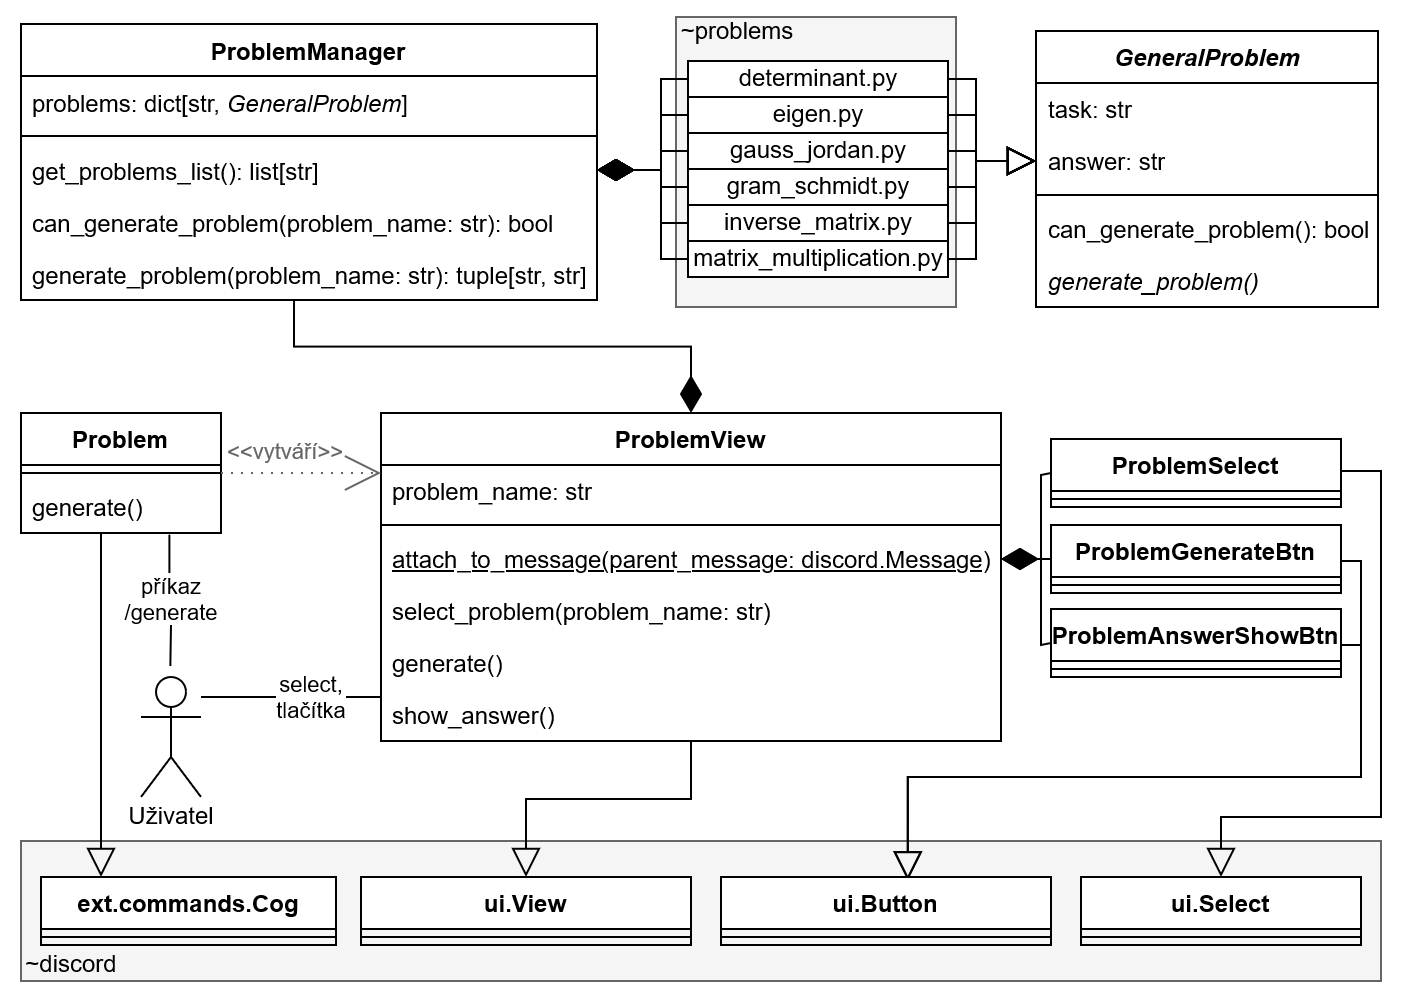
\includegraphics[width=\textwidth]{img/ProblemsDiagram}
		\caption{Diagram tříd generátoru příkladů}
		\label{_tag_img_problemuml}
	\end{figure}
	
	Pro snadné implementování nových kategorií příkladů byla navržena struktura tříd, kterou popisuje obrázek \ref{_tag_img_problemuml}. Abstraktní třída \textit{GeneralProblem} obsahuje řetězce pro zadání a řešení příkladu. Pro jejich nastavení slouží metoda, která je definována v potomcích této třídy. Každý potomek reprezentuje jednu kategorii příkladů a nachází se ve vlastním souboru. Soubory jsou součástí balíku \textit{problems} kvůli snadnějšímu importování. O poskytnutí řetězců k vybrané kategorii se stará \mbox{\textit{ProblemManager}}, který obsahuje všechny potomky \textit{GeneralProblem}. Tato vrchní trojice bloků je nezávislá na platformě Discord a společně s logikou pro vykreslování matematických výrazů by mohla být použita v jakékoliv Python aplikaci.
	
	Spodní část diagramu je závislá na knihovně discord.py. Cog po zadání příkazu odešle zprávu s view, které obsahuje instanci \textit{ProblemManager}. Z ní si view získá seznam dostupných kategorií pro naplnění výběrového seznamu a řetězce se zadáním a řešením, pokud je stisknuto příslušné tlačítko. View se také stará o načtení Markdown souboru s návodem pro výpočet, pokud nějaký existuje.
	
	Do bota byly přidány generátory příkladů pro výpočet násobení matic, soustav rovnic, inverzních matic, vlastních vektorů a determinantu. Příklady pro výpočet soustavy rovnic obsahují tři neznámé a vedou na Gaussovu–Jordanovu eliminační metodu. Příklad tedy začíná maticí s rozměrem 3$\times$3, která musí být převedena na jednotkovou, a tříprvkovým vektorem s výsledky. Pokud by byla počáteční matice vygenerována úplně náhodně, výsledek by pak pravděpodobně obsahoval desetinná čísla, což není pro výukové materiály vhodné. Proto je nejdříve vytvořena jednotková matice, na které je provedeno několik náhodných gaussovských operací, které nemění její lineární obal. Pro snazší kontrolu obsahuje řetězec s řešením kromě výsledku i mezikrok výpočtu, ve kterém je matice v horním stupňovitém tvaru. Pro tento účel je použita metoda LU rozkladu bez zlomků z balíku SymPy. Po použití této metody je ještě každý řádek matice vydělen jeho největším společným dělitelem. Tato podoba matice se totiž nejvíce podobá té, ke které se uživatel dopracuje při ručním výpočtu Gaussovy eliminační metody.
	
	Další kategorií příkladů, kde není vhodné generovat zadání úplně náhodně, je výpočet inverzní matice. V tomto případě je potřeba vygenerovat celočíselnou matici, jejíž inverze je také tvořena celými čísly. Tento požadavek splňují matice, které mají determinant roven $\pm1$. Determinant matice v horním (nebo dolním) stupňovitém tvaru je roven součinu jejích diagonálních prvků a determinant součinu dvou čtvercových matic stejné velikosti je roven součinu determinantů těchto dvou matic \cite{lit_lingebra}. Náhodnou matici, která má determinant roven jedné, tedy lze vytvořit součinem dvou matic, kde jedna je v horním a druhá v dolním stupňovitém tvaru. Obě matice musí mít na diagonále samé jedničky, aby byl jejich determinant roven jedné, a zbylé prvky jsou zvoleny náhodně.
	
	% eigenvalues/eigenvectors
	
	\subsection{Databáze}
	
	\begin{figure}[ht]
		\centering
		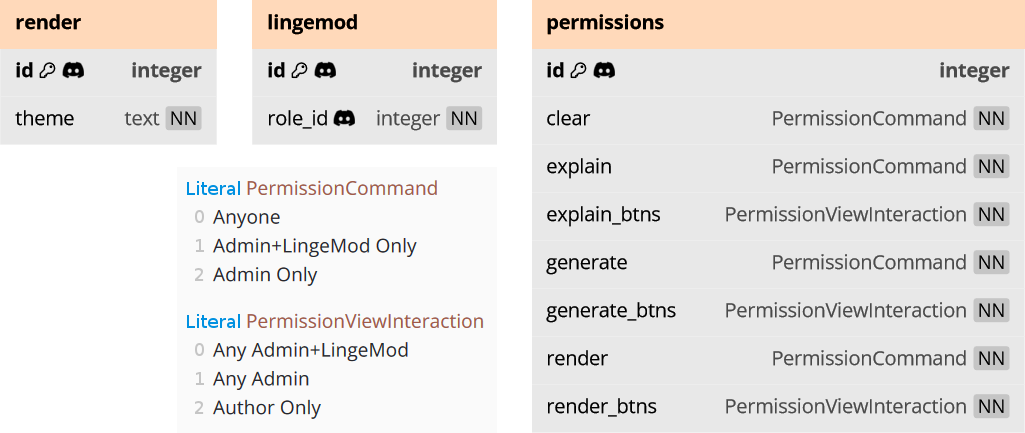
\includegraphics[width=\textwidth]{img/Database}
		\caption{Databáze}
		\label{_tag_img_db}
	\end{figure}
	
	Požadavky bota na databázi nejsou vysoké. Je potřeba ukládat nastavení barevného schématu pro vykreslování matematických výrazů, pokud jej uživatel nebo administrátor změní. Dále je pro každý server, na kterém se bot nachází, ukládán identifikátor moderátorské role LingeMod. Pokud by bot detekoval roli pomocí jejího názvu a role by byla přejmenována, přestala by pak fungovat moderace. Poslední tabulka uchovává nastavení oprávnění pro jednotlivé servery.
	
	Pro takovýto účel byla zvolena databáze SQLite. Mnoho neoficiálních tutoriálů pro tvorbu Discord botů používá jako databázi přímý zápis a čtení ze souborů JSON. Tento způsob je nevhodný, protože není zaručena žádná bezpečnost transakcí a veškerá režie je zanechána na programátorovi. Pokus o implementaci vlastní režie by vedl k naprogramování vlastního databázového systému, proto je vhodnější obrátit se na již hotová a ověřená řešení. SQLite je embedded databáze, která je pro potřeby tohoto bota dostačující a kterou jazyk Python nativně podporuje.
	
	Identifikátory serverů, rolí a uživatelů jsou spravovány na straně Discordu. Každá funkce v knihovně discord.py, která reaguje na událost jako např. zadání příkazu uživatelem, má jako první vstupní parametr objekt typu interakce (\textit{discord.Interaction}), ze kterého lze zjistit ID daného uživatele a serveru, kde byl příkaz zadán. 
	
	Pokud např. uživatel zadá příkaz pro změnu barevného schématu, tak je ID daného serveru získáno z objektu interakce a v tabulce je k němu přiřazen název zvoleného schématu. Pokud je příkaz zadán v přímých zprávách, pak je místo ID serveru, které v tomto kontextu neexistuje, použito ID uživatele. Všechny Discord identifikátory by měly být unikátní, a proto nejsou potřeba dvě tabulky pro schémata serveru a schémata uživatelů. Při použití příkazu \verb|/render| je pak z interakce opět zjištěno ID, pomocí něhož se v databázi dohledá nastavené barevné schéma, které se použije pro vykreslení.
	
	Identifikátory jsou tedy podle potřeby získávány z Discord API. V případě tohoto bota proto může být databáze jednoduchá a tabulky mezi sebou nemusí mít žádné vazby. Definice databáze ze strany SQL obsahuje pouze názvy tabulek a jejich sloupců. Ostatní logika se odehrává na straně programu v jazyce Python.
	
	Pro reprezentaci hodnot uchovávající barevné schéma a oprávnění se používá typ \textit{Literal} z modulu \textit{typing}, který může nabývat jen předem definovaných hodnot. Literal je podporován knihovnou discord.py a pokud je nastaven jako datový typ argumentu příkazu, pak Discord uživateli povolí příkaz odeslat jen tehdy, když je zadaný argument roven některé z předem definovaných hodnot. K hodnotám je navíc dostupné našeptávání.
	
	Typ \textit{ThemeLiteral} může nabývat čtyř různých řetězců, které reprezentují jednotlivá barevná schémata. Tyto řetězce jsou přímo ukládány do databáze k příslušnému ID. U nastavení oprávnění existují dva typy: jeden pro zadání příkazu a druhý pro interakci s tlačítky a výběrovými seznamy. Tyto typy jsou před uložením do databáze převedeny na čísla 0, 1, nebo 2 (viz obrázek \ref{_tag_img_db}). SQLite nepodporuje výčtové typy, a proto se tato konverze opět odehrává na straně hlavního programu.
	
	\subsection{Implementace moderace}
	
	\begin{figure}[ht]
		\centering
		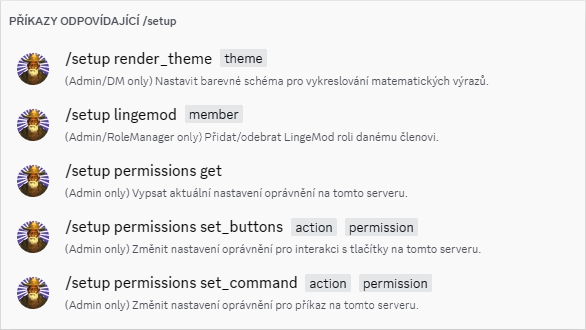
\includegraphics[width=\textwidth]{img/SetupCommands}
		\caption{Seznam příkazů pro nastavení}
	\end{figure}
	
	Příkazy \verb|/setup| jsou součástí tzv. skupiny podpůrných příkazů. Běžný příkaz je zapsán pomocí lomítka, po němž následuje název příkazu, který musí být jednoslovný. Příkazy ze skupiny se zadávají ve tvaru \verb|/<název_skupiny> <název_příkazu>|. Díky tomu mohou mít podobné příkazy stejný začátek a seznam příkazů je tak přehlednější. Skupiny příkazů je možné vnořovat, toho využívají příkazy \verb|/setup permissions|.
	
	Spuštění jednoho z příkazů nastavujících oprávnění změní v tabulce \textit{permissions} na řádku daného serveru příslušný atribut. Záznam v tabulce není přidán hned po připojení bota na server, ale až po prvním spuštění nastavujícího příkazu. Dokud záznam neexistuje, využívá se výchozích hodnot definovaných ve zdrojovém kódu. První volání příkazu nejprve přidá řádek s těmito výchozími hodnotami do tabulky a pak změní vybraný atribut.
	
	Při každém pokusu o spuštění příkazu nebo interakci s view jako první proběhne kontrola oprávnění. Funkce obstarávající tuto kontrolu přistupuje do databáze a má k dispozici objekt interakce, ze kterého lze zjistit údaje o daném uživateli. Pokud má uživatel dostatečná oprávnění, funkce proběhne bez efektu a obsluha jeho interakce může pokračovat. Při nedostatečných právech je vyhozena výjimka, na kterou reaguje cog \textit{on\_error}. Uživateli je v tomto případě odeslána zpráva informující o nedostatečných právech.
	
	Implementace funkce kontroly minimalizuje počet přístupů do databáze. Administrátorům je např. vždy povoleno použít jakýkoliv příkaz nehledě na nastavení oprávnění daného serveru. Nastavení je z databáze získáno až poté, co je z objektu interakce zjištěno, že uživatel administrátorem není. Identifikátor role LingeMod je z databáze získán až v posledním případě, kdy je zjištěno, že příkaz není dostupný všem.
	
	% /setup @app_commands.guild_only : Due to a Discord limitation, this decorator does nothing in subcommands and is ignored.
	% $> lingemod_reset
	% --------------------------------------------------------------------------------------------------------------------------
	% Příkaz /dm
	% $> slash_sync
	% - Problém testování nových funkcí u již nasazeného bota, udělat druhého ? (pak je problém slash commands sync (to by mohly řešit hybridní příkazy (u nich je ale problém ctx vs itx ?)))
		
	\section{Nasazení a zpětná vazba}
	
	Po implementaci všech navrhovaných funkcí byl bot nasazen do testovacího provozu a zpřístupněn skupině uživatelů na otestování. Součástí bylo také dotazníkové šetření, kterého se zúčastnilo celkem devět respondentů.
	
	<< GRAFY DO PŘÍLOHY, ZDE SE K NIM VYJÁDŘIT ? >>
	
	\subsection{Návrhy na vylepšení}
	
	% Jak vylepšit?
	% * Využívat threads nebo nějak lépe spravovat konverzaci, nyní používání bota na větším serveru chaos
	% * generovat sekvence příkladů, "simulace zkoušky"
	% * right click to lingemod, multilang commands (~i témata), search in theory, nějaká vizualizace
	% * Co se týče zápisků z teorie: přidat souvislost s IT
	% * Multilang commands
	% * Kód: Použít SQLAlchemy
	
	\subsection{Vhodnost platformy Discord}
	
	% Vhodnost platformy Discord
	% * Rozdíly mezi PC/web/phone/...
	% * Problém: Discord přestal vykreslovat kurzívu u výrazů jako _f_(_x_), ale *f*(_x_) funguje (za ukončujícím podtržítkem nesmí začínat závorka)
	
	\chapter{Závěr}
	
	Závěr.
	
	% Zdroje
	\chapter*{Seznam použité literatury}
	\addcontentsline{toc}{chapter}{Seznam použité literatury}
	\printbibliography[heading=none]
	
	% Přílohy
	\appendix
	\chapter{Přílohy}
	
	\section{Zdrojové kódy implementace ukázkového příkazu}
	
	\begin{figure}[ht]
		\centering
		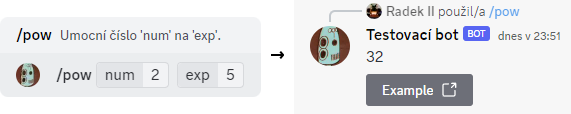
\includegraphics[width=\textwidth]{img/ExampleCommand}
		\caption{Ukázkový příkaz}
		\label{_tag_img_pow}
	\end{figure}
	
	\begin{figure}[ht]
		\lstinputlisting[language=Python3]{code/discord.py}
		\caption{Ukázkový příkaz: Implementace v discord.py}
		\label{_tag_img_discordpy}
	\end{figure}
	
	\begin{figure}[ht]
		\lstinputlisting[language=JavaScript]{code/discord.js}
		\caption{Ukázkový příkaz: Implementace v discord.js}
	\end{figure}
	
	\begin{figure}[ht]
		\lstinputlisting[language={CSharp}]{code/discord.cs}
		\caption{Ukázkový příkaz: Implementace v Discord.Net}
	\end{figure}
	
	\begin{figure}[ht]
		\lstinputlisting[language={Java18}]{code/discord.java}
		\caption{Ukázkový příkaz: Implementace v JDA}
		\label{_tag_img_pow_last}
	\end{figure}
	
\end{document}